\chapter{Full Source Code of the Listing} 
\lstset{style=6502Style}
The listing is so short that it possible (and hopefully not too tedious) for us to
review it in its entirety. This will allow us to understand the basic workings of 
a small 'game' such as this one, from booting to running; it will also give us an
accurate idea of how the final 'Psychedelia' product worked. The difference between
the released game and the listing that appeared in Popular Computing Weekly is not
qualitative - the underlying structure is the same, the core routines we reviewed 
in the previous chapter are more or less identical. The differences lie only in the
the wealth of options available, so it turns out that the listing is an ideal way
for us to get our heads around the core mechanics of the light synthesizer. In the
chapters that follow we can look at some of the features added to the game in more
detail and concentrate on the individual routines that made them work. Here we will
focus instead on the high-level operation of the game and hopefully obtain a sense
of how the thing hangs together.

For the most part I try to present the code in the order it appears in the game
binary itself, but I have moved some routines around here and there so that we're
reading the code in an order that makes sense to the reader.

\clearpage
\begin{lstlisting}
* = $0801
;-----------------------------------------------------
; Start program at CopyCodeToRAM (SYS 2064)
; SYS 2064 ($0810)
;------------------------------------------------------
        .BYTE $0B,$08,$0A,$00
        .BYTE $9E             ; $9E = SYS
        .BYTE $32,$30,$36,$34 ; $32,$30,$36,$34 = 2064
        .BYTE $00,$00,$00,$00,$00,$00
\end{lstlisting}

\bigskip
\bigskip
\bigskip
\bigskip
\bigskip
\bigskip
\bigskip
\bigskip
\begin{lstlisting}
RAM0835LoPtr                        = $FD
RAM0835HiPtr                        = $FE
RAM4000HiPtr                        = $FC
RAM4000LoPtr                        = $FB
;---------------------------------------------------
; CopyCodeToRAM
; Copies the code into position from $0835 to $4000.
;----------------------------------------------------
CopyCodeToRAM
        LDA #$40
        STA RAM4000HiPtr
        LDA #$08
        STA RAM0835HiPtr
        LDA #$00
        STA RAM4000LoPtr
        LDA #$35
        STA RAM0835LoPtr
        LDY #$00
        LDX #$06
CopyLoop   
        LDA (RAM0835LoPtr),Y
        STA (RAM4000LoPtr),Y
        DEY 
        BNE CopyLoop
        INC RAM4000HiPtr
        INC RAM0835HiPtr
        DEX 
        BNE CopyLoop

        JMP InitializeProgram

\end{lstlisting}
\clearpage
\subsubsection{\icode{SYS 2064}}
Yay, let's do some admin like starting the program! All C64 programs begin execution at position \icode{\$0801}, it's the law.
So every C64 program has a little section like this that the C64 executes first and which tells the C64 what to do next.
Here we tell it to start execution at another location \icode{\$0810}. Since we're currently at location \icode{\$0801}, that's
almost 16 bytes ahead and contains the code we've labelled \icode{CopyCodeToRAM} which we jump to next.

The command is given in a slightly strange way. Not strange for the time, but an oddly convoluted convention in its own right.
The \icode{SYS} command is followed by the a series of PETSCII values forming the decimal number 2064. In hexadecimal this is
\icode{\$0810} which is the actual location to start executing. So \icode{SYS 2064} as given by \icode{\$9E \$32\$ 30 \$36,\$34}
means 'start executing whatever is at memory location \icode{\$0810}'. Which in this case is \icode{CopyCodeToRAM}.

\bigskip
\subsubsection{\icode{CopyCodeToRAM}}
Little Commodore 64 programs sure do like copying things around. This routine copies the entire code of the program to a
completely new position in memory at location \icode{\$4000} and then jumps to the routine \icode{InitializeProgram} that will actually start running
'Psychedelia'.

I think this was some sort of cheap and dirty copy protection, designed to prevent people from casually disassembling the
program if they felt minded to do so. 

\clearpage
\begin{lstlisting}
NUM_COLS = $28
NUM_ROWS = $18
;-------------------------------------------------------
; InitializeProgram
;-------------------------------------------------------
InitializeProgram   
        LDA #BLACK
        STA $D020    ;Border Color
        STA $D021    ;Background Color 0

        LDA #>COLOR_RAM
        STA colorRamHiPtr
        LDA #<COLOR_RAM
        STA colorRamLoPtr

        LDX #$00
b4012   LDA colorRamHiPtr
        STA colorRAMLineTableHiPtrArray,X
        LDA colorRamLoPtr
        STA colorRAMLineTableLoPtrArray,X
        CLC 
        ADC #NUM_COLS
        STA colorRamLoPtr
        LDA colorRamHiPtr
        ADC #$00
        STA colorRamHiPtr
        INX 
        CPX #NUM_ROWS+1
        BNE b4012

        JSR InitializeScreenAndText
        JMP LaunchPsychedelia

\end{lstlisting}
\clearpage
\subsubsection{\icode{InitializeProgram}}

More admin!

First we set the background and border color to black.

Next we set up a pair of arrays that Psychedelia will make heavy use of. Together these arrays will function
as a map on to the screen for drawing our pixels. Since the Commodore 64 screen 25 rows high we make the array
25 elements long and each element will contain the address on the screen for the start of each row.

{\color{white}\begin{figure}[H]
  {
    \setlength{\tabcolsep}{3.0pt}
    \setlength\cmidrulewidth{\heavyrulewidth} % Make cmidrule = 
    \begin{adjustbox}{width=11cm,center}
      \begin{tikzpicture}
\fill[c64_black] (0,0) rectangle ++ (1,1);
\fill[c64_black] (1,0) rectangle ++ (1,1);
\fill[c64_black] (2,0) rectangle ++ (1,1);
\fill[c64_black] (3,0) rectangle ++ (1,1);
\fill[c64_black] (4,0) rectangle ++ (1,1);
\fill[c64_black] (5,0) rectangle ++ (1,1);
\fill[c64_black] (6,0) rectangle ++ (1,1);
\fill[c64_black] (7,0) rectangle ++ (1,1);
\fill[c64_black] (8,0) rectangle ++ (1,1);
\fill[c64_black] (9,0) rectangle ++ (1,1);
\fill[c64_black] (10,0) rectangle ++ (1,1);
\fill[c64_black] (11,0) rectangle ++ (1,1);
\fill[c64_black] (12,0) rectangle ++ (1,1);
\fill[c64_black] (13,0) rectangle ++ (1,1);
\fill[c64_black] (14,0) rectangle ++ (1,1);
\fill[c64_black] (15,0) rectangle ++ (1,1);
\fill[c64_black] (16,0) rectangle ++ (1,1);
\fill[c64_black] (17,0) rectangle ++ (1,1);
\fill[c64_black] (18,0) rectangle ++ (1,1);
\fill[c64_black] (19,0) rectangle ++ (1,1);
\fill[c64_black] (20,0) rectangle ++ (1,1);
\fill[c64_black] (21,0) rectangle ++ (1,1);
\fill[c64_black] (22,0) rectangle ++ (1,1);
\fill[c64_black] (23,0) rectangle ++ (1,1);
\fill[c64_black] (24,0) rectangle ++ (1,1);
\fill[c64_black] (25,0) rectangle ++ (1,1);
\fill[c64_black] (26,0) rectangle ++ (1,1);
\fill[c64_black] (27,0) rectangle ++ (1,1);
\fill[c64_black] (28,0) rectangle ++ (1,1);
\fill[c64_black] (29,0) rectangle ++ (1,1);
\fill[c64_black] (30,0) rectangle ++ (1,1);
\fill[c64_black] (31,0) rectangle ++ (1,1);
\fill[c64_black] (32,0) rectangle ++ (1,1);
\fill[c64_black] (33,0) rectangle ++ (1,1);
\fill[c64_black] (34,0) rectangle ++ (1,1);
\fill[c64_black] (35,0) rectangle ++ (1,1);
\fill[c64_black] (36,0) rectangle ++ (1,1);
\fill[c64_black] (37,0) rectangle ++ (1,1);
\fill[c64_black] (38,0) rectangle ++ (1,1);
\fill[c64_black] (39,0) rectangle ++ (1,1);
\fill[c64_black] (0,1) rectangle ++ (1,1);
\fill[c64_black] (1,1) rectangle ++ (1,1);
\fill[c64_black] (2,1) rectangle ++ (1,1);
\fill[c64_black] (3,1) rectangle ++ (1,1);
\fill[c64_black] (4,1) rectangle ++ (1,1);
\fill[c64_black] (5,1) rectangle ++ (1,1);
\fill[c64_black] (6,1) rectangle ++ (1,1);
\fill[c64_black] (7,1) rectangle ++ (1,1);
\fill[c64_black] (8,1) rectangle ++ (1,1);
\fill[c64_black] (9,1) rectangle ++ (1,1);
\fill[c64_black] (10,1) rectangle ++ (1,1);
\fill[c64_black] (11,1) rectangle ++ (1,1);
\fill[c64_black] (12,1) rectangle ++ (1,1);
\fill[c64_black] (13,1) rectangle ++ (1,1);
\fill[c64_black] (14,1) rectangle ++ (1,1);
\fill[c64_black] (15,1) rectangle ++ (1,1);
\fill[c64_black] (16,1) rectangle ++ (1,1);
\fill[c64_black] (17,1) rectangle ++ (1,1);
\fill[c64_black] (18,1) rectangle ++ (1,1);
\fill[c64_black] (19,1) rectangle ++ (1,1);
\fill[c64_black] (20,1) rectangle ++ (1,1);
\fill[c64_black] (21,1) rectangle ++ (1,1);
\fill[c64_black] (22,1) rectangle ++ (1,1);
\fill[c64_black] (23,1) rectangle ++ (1,1);
\fill[c64_black] (24,1) rectangle ++ (1,1);
\fill[c64_black] (25,1) rectangle ++ (1,1);
\fill[c64_black] (26,1) rectangle ++ (1,1);
\fill[c64_black] (27,1) rectangle ++ (1,1);
\fill[c64_black] (28,1) rectangle ++ (1,1);
\fill[c64_black] (29,1) rectangle ++ (1,1);
\fill[c64_black] (30,1) rectangle ++ (1,1);
\fill[c64_black] (31,1) rectangle ++ (1,1);
\fill[c64_black] (32,1) rectangle ++ (1,1);
\fill[c64_black] (33,1) rectangle ++ (1,1);
\fill[c64_black] (34,1) rectangle ++ (1,1);
\fill[c64_black] (35,1) rectangle ++ (1,1);
\fill[c64_black] (36,1) rectangle ++ (1,1);
\fill[c64_black] (37,1) rectangle ++ (1,1);
\fill[c64_black] (38,1) rectangle ++ (1,1);
\fill[c64_black] (39,1) rectangle ++ (1,1);
\fill[c64_black] (0,2) rectangle ++ (1,1);
\fill[c64_black] (1,2) rectangle ++ (1,1);
\fill[c64_black] (2,2) rectangle ++ (1,1);
\fill[c64_black] (3,2) rectangle ++ (1,1);
\fill[c64_black] (4,2) rectangle ++ (1,1);
\fill[c64_black] (5,2) rectangle ++ (1,1);
\fill[c64_black] (6,2) rectangle ++ (1,1);
\fill[c64_black] (7,2) rectangle ++ (1,1);
\fill[c64_black] (8,2) rectangle ++ (1,1);
\fill[c64_black] (9,2) rectangle ++ (1,1);
\fill[c64_black] (10,2) rectangle ++ (1,1);
\fill[c64_black] (11,2) rectangle ++ (1,1);
\fill[c64_black] (12,2) rectangle ++ (1,1);
\fill[c64_black] (13,2) rectangle ++ (1,1);
\fill[c64_black] (14,2) rectangle ++ (1,1);
\fill[c64_black] (15,2) rectangle ++ (1,1);
\fill[c64_black] (16,2) rectangle ++ (1,1);
\fill[c64_black] (17,2) rectangle ++ (1,1);
\fill[c64_black] (18,2) rectangle ++ (1,1);
\fill[c64_black] (19,2) rectangle ++ (1,1);
\fill[c64_black] (20,2) rectangle ++ (1,1);
\fill[c64_black] (21,2) rectangle ++ (1,1);
\fill[c64_black] (22,2) rectangle ++ (1,1);
\fill[c64_black] (23,2) rectangle ++ (1,1);
\fill[c64_black] (24,2) rectangle ++ (1,1);
\fill[c64_black] (25,2) rectangle ++ (1,1);
\fill[c64_black] (26,2) rectangle ++ (1,1);
\fill[c64_black] (27,2) rectangle ++ (1,1);
\fill[c64_black] (28,2) rectangle ++ (1,1);
\fill[c64_black] (29,2) rectangle ++ (1,1);
\fill[c64_black] (30,2) rectangle ++ (1,1);
\fill[c64_black] (31,2) rectangle ++ (1,1);
\fill[c64_black] (32,2) rectangle ++ (1,1);
\fill[c64_black] (33,2) rectangle ++ (1,1);
\fill[c64_black] (34,2) rectangle ++ (1,1);
\fill[c64_black] (35,2) rectangle ++ (1,1);
\fill[c64_black] (36,2) rectangle ++ (1,1);
\fill[c64_black] (37,2) rectangle ++ (1,1);
\fill[c64_black] (38,2) rectangle ++ (1,1);
\fill[c64_black] (39,2) rectangle ++ (1,1);
\fill[c64_black] (0,3) rectangle ++ (1,1);
\fill[c64_black] (1,3) rectangle ++ (1,1);
\fill[c64_black] (2,3) rectangle ++ (1,1);
\fill[c64_black] (3,3) rectangle ++ (1,1);
\fill[c64_black] (4,3) rectangle ++ (1,1);
\fill[c64_black] (5,3) rectangle ++ (1,1);
\fill[c64_black] (6,3) rectangle ++ (1,1);
\fill[c64_black] (7,3) rectangle ++ (1,1);
\fill[c64_black] (8,3) rectangle ++ (1,1);
\fill[c64_black] (9,3) rectangle ++ (1,1);
\fill[c64_black] (10,3) rectangle ++ (1,1);
\fill[c64_black] (11,3) rectangle ++ (1,1);
\fill[c64_black] (12,3) rectangle ++ (1,1);
\fill[c64_black] (13,3) rectangle ++ (1,1);
\fill[c64_black] (14,3) rectangle ++ (1,1);
\fill[c64_black] (15,3) rectangle ++ (1,1);
\fill[c64_black] (16,3) rectangle ++ (1,1);
\fill[c64_black] (17,3) rectangle ++ (1,1);
\fill[c64_black] (18,3) rectangle ++ (1,1);
\fill[c64_black] (19,3) rectangle ++ (1,1);
\fill[c64_black] (20,3) rectangle ++ (1,1);
\fill[c64_black] (21,3) rectangle ++ (1,1);
\fill[c64_black] (22,3) rectangle ++ (1,1);
\fill[c64_black] (23,3) rectangle ++ (1,1);
\fill[c64_black] (24,3) rectangle ++ (1,1);
\fill[c64_black] (25,3) rectangle ++ (1,1);
\fill[c64_black] (26,3) rectangle ++ (1,1);
\fill[c64_black] (27,3) rectangle ++ (1,1);
\fill[c64_black] (28,3) rectangle ++ (1,1);
\fill[c64_black] (29,3) rectangle ++ (1,1);
\fill[c64_black] (30,3) rectangle ++ (1,1);
\fill[c64_black] (31,3) rectangle ++ (1,1);
\fill[c64_black] (32,3) rectangle ++ (1,1);
\fill[c64_black] (33,3) rectangle ++ (1,1);
\fill[c64_black] (34,3) rectangle ++ (1,1);
\fill[c64_black] (35,3) rectangle ++ (1,1);
\fill[c64_black] (36,3) rectangle ++ (1,1);
\fill[c64_black] (37,3) rectangle ++ (1,1);
\fill[c64_black] (38,3) rectangle ++ (1,1);
\fill[c64_black] (39,3) rectangle ++ (1,1);
\fill[c64_black] (0,4) rectangle ++ (1,1);
\fill[c64_black] (1,4) rectangle ++ (1,1);
\fill[c64_black] (2,4) rectangle ++ (1,1);
\fill[c64_black] (3,4) rectangle ++ (1,1);
\fill[c64_black] (4,4) rectangle ++ (1,1);
\fill[c64_black] (5,4) rectangle ++ (1,1);
\fill[c64_black] (6,4) rectangle ++ (1,1);
\fill[c64_black] (7,4) rectangle ++ (1,1);
\fill[c64_black] (8,4) rectangle ++ (1,1);
\fill[c64_black] (9,4) rectangle ++ (1,1);
\fill[c64_black] (10,4) rectangle ++ (1,1);
\fill[c64_black] (11,4) rectangle ++ (1,1);
\fill[c64_black] (12,4) rectangle ++ (1,1);
\fill[c64_black] (13,4) rectangle ++ (1,1);
\fill[c64_black] (14,4) rectangle ++ (1,1);
\fill[c64_black] (15,4) rectangle ++ (1,1);
\fill[c64_black] (16,4) rectangle ++ (1,1);
\fill[c64_black] (17,4) rectangle ++ (1,1);
\fill[c64_black] (18,4) rectangle ++ (1,1);
\fill[c64_black] (19,4) rectangle ++ (1,1);
\fill[c64_black] (20,4) rectangle ++ (1,1);
\fill[c64_black] (21,4) rectangle ++ (1,1);
\fill[c64_black] (22,4) rectangle ++ (1,1);
\fill[c64_black] (23,4) rectangle ++ (1,1);
\fill[c64_black] (24,4) rectangle ++ (1,1);
\fill[c64_black] (25,4) rectangle ++ (1,1);
\fill[c64_black] (26,4) rectangle ++ (1,1);
\fill[c64_black] (27,4) rectangle ++ (1,1);
\fill[c64_black] (28,4) rectangle ++ (1,1);
\fill[c64_black] (29,4) rectangle ++ (1,1);
\fill[c64_black] (30,4) rectangle ++ (1,1);
\fill[c64_black] (31,4) rectangle ++ (1,1);
\fill[c64_black] (32,4) rectangle ++ (1,1);
\fill[c64_black] (33,4) rectangle ++ (1,1);
\fill[c64_black] (34,4) rectangle ++ (1,1);
\fill[c64_black] (35,4) rectangle ++ (1,1);
\fill[c64_black] (36,4) rectangle ++ (1,1);
\fill[c64_black] (37,4) rectangle ++ (1,1);
\fill[c64_black] (38,4) rectangle ++ (1,1);
\fill[c64_black] (39,4) rectangle ++ (1,1);
\fill[c64_black] (0,5) rectangle ++ (1,1);
\fill[c64_black] (1,5) rectangle ++ (1,1);
\fill[c64_black] (2,5) rectangle ++ (1,1);
\fill[c64_black] (3,5) rectangle ++ (1,1);
\fill[c64_black] (4,5) rectangle ++ (1,1);
\fill[c64_black] (5,5) rectangle ++ (1,1);
\fill[c64_black] (6,5) rectangle ++ (1,1);
\fill[c64_black] (7,5) rectangle ++ (1,1);
\fill[c64_black] (8,5) rectangle ++ (1,1);
\fill[c64_black] (9,5) rectangle ++ (1,1);
\fill[c64_black] (10,5) rectangle ++ (1,1);
\fill[c64_black] (11,5) rectangle ++ (1,1);
\fill[c64_black] (12,5) rectangle ++ (1,1);
\fill[c64_black] (13,5) rectangle ++ (1,1);
\fill[c64_black] (14,5) rectangle ++ (1,1);
\fill[c64_black] (15,5) rectangle ++ (1,1);
\fill[c64_black] (16,5) rectangle ++ (1,1);
\fill[c64_black] (17,5) rectangle ++ (1,1);
\fill[c64_black] (18,5) rectangle ++ (1,1);
\fill[c64_black] (19,5) rectangle ++ (1,1);
\fill[c64_black] (20,5) rectangle ++ (1,1);
\fill[c64_black] (21,5) rectangle ++ (1,1);
\fill[c64_black] (22,5) rectangle ++ (1,1);
\fill[c64_black] (23,5) rectangle ++ (1,1);
\fill[c64_black] (24,5) rectangle ++ (1,1);
\fill[c64_black] (25,5) rectangle ++ (1,1);
\fill[c64_black] (26,5) rectangle ++ (1,1);
\fill[c64_black] (27,5) rectangle ++ (1,1);
\fill[c64_black] (28,5) rectangle ++ (1,1);
\fill[c64_black] (29,5) rectangle ++ (1,1);
\fill[c64_black] (30,5) rectangle ++ (1,1);
\fill[c64_black] (31,5) rectangle ++ (1,1);
\fill[c64_black] (32,5) rectangle ++ (1,1);
\fill[c64_black] (33,5) rectangle ++ (1,1);
\fill[c64_black] (34,5) rectangle ++ (1,1);
\fill[c64_black] (35,5) rectangle ++ (1,1);
\fill[c64_black] (36,5) rectangle ++ (1,1);
\fill[c64_black] (37,5) rectangle ++ (1,1);
\fill[c64_black] (38,5) rectangle ++ (1,1);
\fill[c64_black] (39,5) rectangle ++ (1,1);
\fill[c64_black] (0,6) rectangle ++ (1,1);
\fill[c64_black] (1,6) rectangle ++ (1,1);
\fill[c64_black] (2,6) rectangle ++ (1,1);
\fill[c64_black] (3,6) rectangle ++ (1,1);
\fill[c64_black] (4,6) rectangle ++ (1,1);
\fill[c64_black] (5,6) rectangle ++ (1,1);
\fill[c64_black] (6,6) rectangle ++ (1,1);
\fill[c64_black] (7,6) rectangle ++ (1,1);
\fill[c64_black] (8,6) rectangle ++ (1,1);
\fill[c64_black] (9,6) rectangle ++ (1,1);
\fill[c64_black] (10,6) rectangle ++ (1,1);
\fill[c64_black] (11,6) rectangle ++ (1,1);
\fill[c64_black] (12,6) rectangle ++ (1,1);
\fill[c64_black] (13,6) rectangle ++ (1,1);
\fill[c64_black] (14,6) rectangle ++ (1,1);
\fill[c64_black] (15,6) rectangle ++ (1,1);
\fill[c64_black] (16,6) rectangle ++ (1,1);
\fill[c64_black] (17,6) rectangle ++ (1,1);
\fill[c64_black] (18,6) rectangle ++ (1,1);
\fill[c64_black] (19,6) rectangle ++ (1,1);
\fill[c64_black] (20,6) rectangle ++ (1,1);
\fill[c64_black] (21,6) rectangle ++ (1,1);
\fill[c64_black] (22,6) rectangle ++ (1,1);
\fill[c64_black] (23,6) rectangle ++ (1,1);
\fill[c64_black] (24,6) rectangle ++ (1,1);
\fill[c64_black] (25,6) rectangle ++ (1,1);
\fill[c64_black] (26,6) rectangle ++ (1,1);
\fill[c64_black] (27,6) rectangle ++ (1,1);
\fill[c64_black] (28,6) rectangle ++ (1,1);
\fill[c64_black] (29,6) rectangle ++ (1,1);
\fill[c64_black] (30,6) rectangle ++ (1,1);
\fill[c64_black] (31,6) rectangle ++ (1,1);
\fill[c64_black] (32,6) rectangle ++ (1,1);
\fill[c64_black] (33,6) rectangle ++ (1,1);
\fill[c64_black] (34,6) rectangle ++ (1,1);
\fill[c64_black] (35,6) rectangle ++ (1,1);
\fill[c64_black] (36,6) rectangle ++ (1,1);
\fill[c64_black] (37,6) rectangle ++ (1,1);
\fill[c64_black] (38,6) rectangle ++ (1,1);
\fill[c64_black] (39,6) rectangle ++ (1,1);
\fill[c64_black] (0,7) rectangle ++ (1,1);
\fill[c64_black] (1,7) rectangle ++ (1,1);
\fill[c64_black] (2,7) rectangle ++ (1,1);
\fill[c64_black] (3,7) rectangle ++ (1,1);
\fill[c64_black] (4,7) rectangle ++ (1,1);
\fill[c64_black] (5,7) rectangle ++ (1,1);
\fill[c64_black] (6,7) rectangle ++ (1,1);
\fill[c64_black] (7,7) rectangle ++ (1,1);
\fill[c64_black] (8,7) rectangle ++ (1,1);
\fill[c64_black] (9,7) rectangle ++ (1,1);
\fill[c64_black] (10,7) rectangle ++ (1,1);
\fill[c64_black] (11,7) rectangle ++ (1,1);
\fill[c64_black] (12,7) rectangle ++ (1,1);
\fill[c64_black] (13,7) rectangle ++ (1,1);
\fill[c64_black] (14,7) rectangle ++ (1,1);
\fill[c64_black] (15,7) rectangle ++ (1,1);
\fill[c64_black] (16,7) rectangle ++ (1,1);
\fill[c64_red] (17,7) rectangle ++ (1,1);
\fill[c64_black] (18,7) rectangle ++ (1,1);
\fill[c64_red] (19,7) rectangle ++ (1,1);
\fill[c64_black] (20,7) rectangle ++ (1,1);
\fill[c64_black] (21,7) rectangle ++ (1,1);
\fill[c64_black] (22,7) rectangle ++ (1,1);
\fill[c64_black] (23,7) rectangle ++ (1,1);
\fill[c64_black] (24,7) rectangle ++ (1,1);
\fill[c64_black] (25,7) rectangle ++ (1,1);
\fill[c64_black] (26,7) rectangle ++ (1,1);
\fill[c64_black] (27,7) rectangle ++ (1,1);
\fill[c64_black] (28,7) rectangle ++ (1,1);
\fill[c64_black] (29,7) rectangle ++ (1,1);
\fill[c64_black] (30,7) rectangle ++ (1,1);
\fill[c64_black] (31,7) rectangle ++ (1,1);
\fill[c64_black] (32,7) rectangle ++ (1,1);
\fill[c64_black] (33,7) rectangle ++ (1,1);
\fill[c64_black] (34,7) rectangle ++ (1,1);
\fill[c64_black] (35,7) rectangle ++ (1,1);
\fill[c64_black] (36,7) rectangle ++ (1,1);
\fill[c64_black] (37,7) rectangle ++ (1,1);
\fill[c64_black] (38,7) rectangle ++ (1,1);
\fill[c64_black] (39,7) rectangle ++ (1,1);
\fill[c64_black] (0,8) rectangle ++ (1,1);
\fill[c64_black] (1,8) rectangle ++ (1,1);
\fill[c64_black] (2,8) rectangle ++ (1,1);
\fill[c64_black] (3,8) rectangle ++ (1,1);
\fill[c64_black] (4,8) rectangle ++ (1,1);
\fill[c64_black] (5,8) rectangle ++ (1,1);
\fill[c64_black] (6,8) rectangle ++ (1,1);
\fill[c64_black] (7,8) rectangle ++ (1,1);
\fill[c64_black] (8,8) rectangle ++ (1,1);
\fill[c64_black] (9,8) rectangle ++ (1,1);
\fill[c64_black] (10,8) rectangle ++ (1,1);
\fill[c64_black] (11,8) rectangle ++ (1,1);
\fill[c64_black] (12,8) rectangle ++ (1,1);
\fill[c64_black] (13,8) rectangle ++ (1,1);
\fill[c64_black] (14,8) rectangle ++ (1,1);
\fill[c64_black] (15,8) rectangle ++ (1,1);
\fill[c64_black] (16,8) rectangle ++ (1,1);
\fill[c64_black] (17,8) rectangle ++ (1,1);
\fill[c64_red] (18,8) rectangle ++ (1,1);
\fill[c64_black] (19,8) rectangle ++ (1,1);
\fill[c64_black] (20,8) rectangle ++ (1,1);
\fill[c64_black] (21,8) rectangle ++ (1,1);
\fill[c64_black] (22,8) rectangle ++ (1,1);
\fill[c64_black] (23,8) rectangle ++ (1,1);
\fill[c64_black] (24,8) rectangle ++ (1,1);
\fill[c64_black] (25,8) rectangle ++ (1,1);
\fill[c64_black] (26,8) rectangle ++ (1,1);
\fill[c64_black] (27,8) rectangle ++ (1,1);
\fill[c64_black] (28,8) rectangle ++ (1,1);
\fill[c64_black] (29,8) rectangle ++ (1,1);
\fill[c64_black] (30,8) rectangle ++ (1,1);
\fill[c64_black] (31,8) rectangle ++ (1,1);
\fill[c64_black] (32,8) rectangle ++ (1,1);
\fill[c64_black] (33,8) rectangle ++ (1,1);
\fill[c64_black] (34,8) rectangle ++ (1,1);
\fill[c64_black] (35,8) rectangle ++ (1,1);
\fill[c64_black] (36,8) rectangle ++ (1,1);
\fill[c64_black] (37,8) rectangle ++ (1,1);
\fill[c64_black] (38,8) rectangle ++ (1,1);
\fill[c64_black] (39,8) rectangle ++ (1,1);
\fill[c64_black] (0,9) rectangle ++ (1,1);
\fill[c64_black] (1,9) rectangle ++ (1,1);
\fill[c64_black] (2,9) rectangle ++ (1,1);
\fill[c64_black] (3,9) rectangle ++ (1,1);
\fill[c64_black] (4,9) rectangle ++ (1,1);
\fill[c64_black] (5,9) rectangle ++ (1,1);
\fill[c64_black] (6,9) rectangle ++ (1,1);
\fill[c64_black] (7,9) rectangle ++ (1,1);
\fill[c64_black] (8,9) rectangle ++ (1,1);
\fill[c64_black] (9,9) rectangle ++ (1,1);
\fill[c64_black] (10,9) rectangle ++ (1,1);
\fill[c64_black] (11,9) rectangle ++ (1,1);
\fill[c64_black] (12,9) rectangle ++ (1,1);
\fill[c64_black] (13,9) rectangle ++ (1,1);
\fill[c64_black] (14,9) rectangle ++ (1,1);
\fill[c64_black] (15,9) rectangle ++ (1,1);
\fill[c64_black] (16,9) rectangle ++ (1,1);
\fill[c64_black] (17,9) rectangle ++ (1,1);
\fill[c64_green] (18,9) rectangle ++ (1,1);
\fill[c64_black] (19,9) rectangle ++ (1,1);
\fill[c64_black] (20,9) rectangle ++ (1,1);
\fill[c64_black] (21,9) rectangle ++ (1,1);
\fill[c64_black] (22,9) rectangle ++ (1,1);
\fill[c64_black] (23,9) rectangle ++ (1,1);
\fill[c64_black] (24,9) rectangle ++ (1,1);
\fill[c64_black] (25,9) rectangle ++ (1,1);
\fill[c64_black] (26,9) rectangle ++ (1,1);
\fill[c64_black] (27,9) rectangle ++ (1,1);
\fill[c64_black] (28,9) rectangle ++ (1,1);
\fill[c64_black] (29,9) rectangle ++ (1,1);
\fill[c64_black] (30,9) rectangle ++ (1,1);
\fill[c64_black] (31,9) rectangle ++ (1,1);
\fill[c64_black] (32,9) rectangle ++ (1,1);
\fill[c64_black] (33,9) rectangle ++ (1,1);
\fill[c64_black] (34,9) rectangle ++ (1,1);
\fill[c64_black] (35,9) rectangle ++ (1,1);
\fill[c64_black] (36,9) rectangle ++ (1,1);
\fill[c64_black] (37,9) rectangle ++ (1,1);
\fill[c64_black] (38,9) rectangle ++ (1,1);
\fill[c64_black] (39,9) rectangle ++ (1,1);
\fill[c64_black] (0,10) rectangle ++ (1,1);
\fill[c64_black] (1,10) rectangle ++ (1,1);
\fill[c64_black] (2,10) rectangle ++ (1,1);
\fill[c64_black] (3,10) rectangle ++ (1,1);
\fill[c64_black] (4,10) rectangle ++ (1,1);
\fill[c64_black] (5,10) rectangle ++ (1,1);
\fill[c64_black] (6,10) rectangle ++ (1,1);
\fill[c64_black] (7,10) rectangle ++ (1,1);
\fill[c64_black] (8,10) rectangle ++ (1,1);
\fill[c64_black] (9,10) rectangle ++ (1,1);
\fill[c64_black] (10,10) rectangle ++ (1,1);
\fill[c64_black] (11,10) rectangle ++ (1,1);
\fill[c64_black] (12,10) rectangle ++ (1,1);
\fill[c64_black] (13,10) rectangle ++ (1,1);
\fill[c64_black] (14,10) rectangle ++ (1,1);
\fill[c64_black] (15,10) rectangle ++ (1,1);
\fill[c64_black] (16,10) rectangle ++ (1,1);
\fill[c64_black] (17,10) rectangle ++ (1,1);
\fill[c64_cyan] (18,10) rectangle ++ (1,1);
\fill[c64_black] (19,10) rectangle ++ (1,1);
\fill[c64_black] (20,10) rectangle ++ (1,1);
\fill[c64_black] (21,10) rectangle ++ (1,1);
\fill[c64_black] (22,10) rectangle ++ (1,1);
\fill[c64_black] (23,10) rectangle ++ (1,1);
\fill[c64_black] (24,10) rectangle ++ (1,1);
\fill[c64_black] (25,10) rectangle ++ (1,1);
\fill[c64_black] (26,10) rectangle ++ (1,1);
\fill[c64_black] (27,10) rectangle ++ (1,1);
\fill[c64_black] (28,10) rectangle ++ (1,1);
\fill[c64_black] (29,10) rectangle ++ (1,1);
\fill[c64_black] (30,10) rectangle ++ (1,1);
\fill[c64_black] (31,10) rectangle ++ (1,1);
\fill[c64_black] (32,10) rectangle ++ (1,1);
\fill[c64_black] (33,10) rectangle ++ (1,1);
\fill[c64_black] (34,10) rectangle ++ (1,1);
\fill[c64_black] (35,10) rectangle ++ (1,1);
\fill[c64_black] (36,10) rectangle ++ (1,1);
\fill[c64_black] (37,10) rectangle ++ (1,1);
\fill[c64_black] (38,10) rectangle ++ (1,1);
\fill[c64_black] (39,10) rectangle ++ (1,1);
\fill[c64_black] (0,11) rectangle ++ (1,1);
\fill[c64_black] (1,11) rectangle ++ (1,1);
\fill[c64_black] (2,11) rectangle ++ (1,1);
\fill[c64_black] (3,11) rectangle ++ (1,1);
\fill[c64_black] (4,11) rectangle ++ (1,1);
\fill[c64_black] (5,11) rectangle ++ (1,1);
\fill[c64_black] (6,11) rectangle ++ (1,1);
\fill[c64_black] (7,11) rectangle ++ (1,1);
\fill[c64_black] (8,11) rectangle ++ (1,1);
\fill[c64_black] (9,11) rectangle ++ (1,1);
\fill[c64_black] (10,11) rectangle ++ (1,1);
\fill[c64_black] (11,11) rectangle ++ (1,1);
\fill[c64_black] (12,11) rectangle ++ (1,1);
\fill[c64_red] (13,11) rectangle ++ (1,1);
\fill[c64_black] (14,11) rectangle ++ (1,1);
\fill[c64_black] (15,11) rectangle ++ (1,1);
\fill[c64_black] (16,11) rectangle ++ (1,1);
\fill[c64_yellow] (17,11) rectangle ++ (1,1);
\fill[c64_yellow] (18,11) rectangle ++ (1,1);
\fill[c64_yellow] (19,11) rectangle ++ (1,1);
\fill[c64_black] (20,11) rectangle ++ (1,1);
\fill[c64_black] (21,11) rectangle ++ (1,1);
\fill[c64_black] (22,11) rectangle ++ (1,1);
\fill[c64_red] (23,11) rectangle ++ (1,1);
\fill[c64_black] (24,11) rectangle ++ (1,1);
\fill[c64_black] (25,11) rectangle ++ (1,1);
\fill[c64_black] (26,11) rectangle ++ (1,1);
\fill[c64_black] (27,11) rectangle ++ (1,1);
\fill[c64_black] (28,11) rectangle ++ (1,1);
\fill[c64_black] (29,11) rectangle ++ (1,1);
\fill[c64_black] (30,11) rectangle ++ (1,1);
\fill[c64_black] (31,11) rectangle ++ (1,1);
\fill[c64_black] (32,11) rectangle ++ (1,1);
\fill[c64_black] (33,11) rectangle ++ (1,1);
\fill[c64_black] (34,11) rectangle ++ (1,1);
\fill[c64_black] (35,11) rectangle ++ (1,1);
\fill[c64_black] (36,11) rectangle ++ (1,1);
\fill[c64_black] (37,11) rectangle ++ (1,1);
\fill[c64_black] (38,11) rectangle ++ (1,1);
\fill[c64_black] (39,11) rectangle ++ (1,1);
\fill[c64_black] (0,12) rectangle ++ (1,1);
\fill[c64_black] (1,12) rectangle ++ (1,1);
\fill[c64_black] (2,12) rectangle ++ (1,1);
\fill[c64_black] (3,12) rectangle ++ (1,1);
\fill[c64_black] (4,12) rectangle ++ (1,1);
\fill[c64_black] (5,12) rectangle ++ (1,1);
\fill[c64_black] (6,12) rectangle ++ (1,1);
\fill[c64_black] (7,12) rectangle ++ (1,1);
\fill[c64_black] (8,12) rectangle ++ (1,1);
\fill[c64_black] (9,12) rectangle ++ (1,1);
\fill[c64_black] (10,12) rectangle ++ (1,1);
\fill[c64_black] (11,12) rectangle ++ (1,1);
\fill[c64_black] (12,12) rectangle ++ (1,1);
\fill[c64_black] (13,12) rectangle ++ (1,1);
\fill[c64_red] (14,12) rectangle ++ (1,1);
\fill[c64_green] (15,12) rectangle ++ (1,1);
\fill[c64_cyan] (16,12) rectangle ++ (1,1);
\fill[c64_yellow] (17,12) rectangle ++ (1,1);
\fill[c64_yellow] (18,12) rectangle ++ (1,1);
\fill[c64_yellow] (19,12) rectangle ++ (1,1);
\fill[c64_cyan] (20,12) rectangle ++ (1,1);
\fill[c64_green] (21,12) rectangle ++ (1,1);
\fill[c64_red] (22,12) rectangle ++ (1,1);
\fill[c64_black] (23,12) rectangle ++ (1,1);
\fill[c64_black] (24,12) rectangle ++ (1,1);
\fill[c64_black] (25,12) rectangle ++ (1,1);
\fill[c64_black] (26,12) rectangle ++ (1,1);
\fill[c64_black] (27,12) rectangle ++ (1,1);
\fill[c64_black] (28,12) rectangle ++ (1,1);
\fill[c64_black] (29,12) rectangle ++ (1,1);
\fill[c64_black] (30,12) rectangle ++ (1,1);
\fill[c64_black] (31,12) rectangle ++ (1,1);
\fill[c64_black] (32,12) rectangle ++ (1,1);
\fill[c64_black] (33,12) rectangle ++ (1,1);
\fill[c64_black] (34,12) rectangle ++ (1,1);
\fill[c64_black] (35,12) rectangle ++ (1,1);
\fill[c64_black] (36,12) rectangle ++ (1,1);
\fill[c64_black] (37,12) rectangle ++ (1,1);
\fill[c64_black] (38,12) rectangle ++ (1,1);
\fill[c64_black] (39,12) rectangle ++ (1,1);
\fill[c64_black] (0,13) rectangle ++ (1,1);
\fill[c64_black] (1,13) rectangle ++ (1,1);
\fill[c64_black] (2,13) rectangle ++ (1,1);
\fill[c64_black] (3,13) rectangle ++ (1,1);
\fill[c64_black] (4,13) rectangle ++ (1,1);
\fill[c64_black] (5,13) rectangle ++ (1,1);
\fill[c64_black] (6,13) rectangle ++ (1,1);
\fill[c64_black] (7,13) rectangle ++ (1,1);
\fill[c64_black] (8,13) rectangle ++ (1,1);
\fill[c64_black] (9,13) rectangle ++ (1,1);
\fill[c64_black] (10,13) rectangle ++ (1,1);
\fill[c64_black] (11,13) rectangle ++ (1,1);
\fill[c64_black] (12,13) rectangle ++ (1,1);
\fill[c64_red] (13,13) rectangle ++ (1,1);
\fill[c64_black] (14,13) rectangle ++ (1,1);
\fill[c64_black] (15,13) rectangle ++ (1,1);
\fill[c64_black] (16,13) rectangle ++ (1,1);
\fill[c64_yellow] (17,13) rectangle ++ (1,1);
\fill[c64_yellow] (18,13) rectangle ++ (1,1);
\fill[c64_yellow] (19,13) rectangle ++ (1,1);
\fill[c64_black] (20,13) rectangle ++ (1,1);
\fill[c64_black] (21,13) rectangle ++ (1,1);
\fill[c64_black] (22,13) rectangle ++ (1,1);
\fill[c64_red] (23,13) rectangle ++ (1,1);
\fill[c64_black] (24,13) rectangle ++ (1,1);
\fill[c64_black] (25,13) rectangle ++ (1,1);
\fill[c64_black] (26,13) rectangle ++ (1,1);
\fill[c64_black] (27,13) rectangle ++ (1,1);
\fill[c64_black] (28,13) rectangle ++ (1,1);
\fill[c64_black] (29,13) rectangle ++ (1,1);
\fill[c64_black] (30,13) rectangle ++ (1,1);
\fill[c64_black] (31,13) rectangle ++ (1,1);
\fill[c64_black] (32,13) rectangle ++ (1,1);
\fill[c64_black] (33,13) rectangle ++ (1,1);
\fill[c64_black] (34,13) rectangle ++ (1,1);
\fill[c64_black] (35,13) rectangle ++ (1,1);
\fill[c64_black] (36,13) rectangle ++ (1,1);
\fill[c64_black] (37,13) rectangle ++ (1,1);
\fill[c64_black] (38,13) rectangle ++ (1,1);
\fill[c64_black] (39,13) rectangle ++ (1,1);
\fill[c64_black] (0,14) rectangle ++ (1,1);
\fill[c64_black] (1,14) rectangle ++ (1,1);
\fill[c64_black] (2,14) rectangle ++ (1,1);
\fill[c64_black] (3,14) rectangle ++ (1,1);
\fill[c64_black] (4,14) rectangle ++ (1,1);
\fill[c64_black] (5,14) rectangle ++ (1,1);
\fill[c64_black] (6,14) rectangle ++ (1,1);
\fill[c64_black] (7,14) rectangle ++ (1,1);
\fill[c64_black] (8,14) rectangle ++ (1,1);
\fill[c64_black] (9,14) rectangle ++ (1,1);
\fill[c64_black] (10,14) rectangle ++ (1,1);
\fill[c64_black] (11,14) rectangle ++ (1,1);
\fill[c64_black] (12,14) rectangle ++ (1,1);
\fill[c64_black] (13,14) rectangle ++ (1,1);
\fill[c64_black] (14,14) rectangle ++ (1,1);
\fill[c64_black] (15,14) rectangle ++ (1,1);
\fill[c64_black] (16,14) rectangle ++ (1,1);
\fill[c64_black] (17,14) rectangle ++ (1,1);
\fill[c64_cyan] (18,14) rectangle ++ (1,1);
\fill[c64_black] (19,14) rectangle ++ (1,1);
\fill[c64_black] (20,14) rectangle ++ (1,1);
\fill[c64_black] (21,14) rectangle ++ (1,1);
\fill[c64_black] (22,14) rectangle ++ (1,1);
\fill[c64_black] (23,14) rectangle ++ (1,1);
\fill[c64_black] (24,14) rectangle ++ (1,1);
\fill[c64_black] (25,14) rectangle ++ (1,1);
\fill[c64_black] (26,14) rectangle ++ (1,1);
\fill[c64_black] (27,14) rectangle ++ (1,1);
\fill[c64_black] (28,14) rectangle ++ (1,1);
\fill[c64_black] (29,14) rectangle ++ (1,1);
\fill[c64_black] (30,14) rectangle ++ (1,1);
\fill[c64_black] (31,14) rectangle ++ (1,1);
\fill[c64_black] (32,14) rectangle ++ (1,1);
\fill[c64_black] (33,14) rectangle ++ (1,1);
\fill[c64_black] (34,14) rectangle ++ (1,1);
\fill[c64_black] (35,14) rectangle ++ (1,1);
\fill[c64_black] (36,14) rectangle ++ (1,1);
\fill[c64_black] (37,14) rectangle ++ (1,1);
\fill[c64_black] (38,14) rectangle ++ (1,1);
\fill[c64_black] (39,14) rectangle ++ (1,1);
\fill[c64_black] (0,15) rectangle ++ (1,1);
\fill[c64_black] (1,15) rectangle ++ (1,1);
\fill[c64_black] (2,15) rectangle ++ (1,1);
\fill[c64_black] (3,15) rectangle ++ (1,1);
\fill[c64_black] (4,15) rectangle ++ (1,1);
\fill[c64_black] (5,15) rectangle ++ (1,1);
\fill[c64_black] (6,15) rectangle ++ (1,1);
\fill[c64_black] (7,15) rectangle ++ (1,1);
\fill[c64_black] (8,15) rectangle ++ (1,1);
\fill[c64_black] (9,15) rectangle ++ (1,1);
\fill[c64_black] (10,15) rectangle ++ (1,1);
\fill[c64_black] (11,15) rectangle ++ (1,1);
\fill[c64_black] (12,15) rectangle ++ (1,1);
\fill[c64_black] (13,15) rectangle ++ (1,1);
\fill[c64_black] (14,15) rectangle ++ (1,1);
\fill[c64_black] (15,15) rectangle ++ (1,1);
\fill[c64_black] (16,15) rectangle ++ (1,1);
\fill[c64_black] (17,15) rectangle ++ (1,1);
\fill[c64_green] (18,15) rectangle ++ (1,1);
\fill[c64_black] (19,15) rectangle ++ (1,1);
\fill[c64_black] (20,15) rectangle ++ (1,1);
\fill[c64_black] (21,15) rectangle ++ (1,1);
\fill[c64_black] (22,15) rectangle ++ (1,1);
\fill[c64_black] (23,15) rectangle ++ (1,1);
\fill[c64_black] (24,15) rectangle ++ (1,1);
\fill[c64_black] (25,15) rectangle ++ (1,1);
\fill[c64_black] (26,15) rectangle ++ (1,1);
\fill[c64_black] (27,15) rectangle ++ (1,1);
\fill[c64_black] (28,15) rectangle ++ (1,1);
\fill[c64_black] (29,15) rectangle ++ (1,1);
\fill[c64_black] (30,15) rectangle ++ (1,1);
\fill[c64_black] (31,15) rectangle ++ (1,1);
\fill[c64_black] (32,15) rectangle ++ (1,1);
\fill[c64_black] (33,15) rectangle ++ (1,1);
\fill[c64_black] (34,15) rectangle ++ (1,1);
\fill[c64_black] (35,15) rectangle ++ (1,1);
\fill[c64_black] (36,15) rectangle ++ (1,1);
\fill[c64_black] (37,15) rectangle ++ (1,1);
\fill[c64_black] (38,15) rectangle ++ (1,1);
\fill[c64_black] (39,15) rectangle ++ (1,1);
\fill[c64_black] (0,16) rectangle ++ (1,1);
\fill[c64_black] (1,16) rectangle ++ (1,1);
\fill[c64_black] (2,16) rectangle ++ (1,1);
\fill[c64_black] (3,16) rectangle ++ (1,1);
\fill[c64_black] (4,16) rectangle ++ (1,1);
\fill[c64_black] (5,16) rectangle ++ (1,1);
\fill[c64_black] (6,16) rectangle ++ (1,1);
\fill[c64_black] (7,16) rectangle ++ (1,1);
\fill[c64_black] (8,16) rectangle ++ (1,1);
\fill[c64_black] (9,16) rectangle ++ (1,1);
\fill[c64_black] (10,16) rectangle ++ (1,1);
\fill[c64_black] (11,16) rectangle ++ (1,1);
\fill[c64_black] (12,16) rectangle ++ (1,1);
\fill[c64_black] (13,16) rectangle ++ (1,1);
\fill[c64_black] (14,16) rectangle ++ (1,1);
\fill[c64_black] (15,16) rectangle ++ (1,1);
\fill[c64_black] (16,16) rectangle ++ (1,1);
\fill[c64_black] (17,16) rectangle ++ (1,1);
\fill[c64_red] (18,16) rectangle ++ (1,1);
\fill[c64_black] (19,16) rectangle ++ (1,1);
\fill[c64_black] (20,16) rectangle ++ (1,1);
\fill[c64_black] (21,16) rectangle ++ (1,1);
\fill[c64_black] (22,16) rectangle ++ (1,1);
\fill[c64_black] (23,16) rectangle ++ (1,1);
\fill[c64_black] (24,16) rectangle ++ (1,1);
\fill[c64_black] (25,16) rectangle ++ (1,1);
\fill[c64_black] (26,16) rectangle ++ (1,1);
\fill[c64_black] (27,16) rectangle ++ (1,1);
\fill[c64_black] (28,16) rectangle ++ (1,1);
\fill[c64_black] (29,16) rectangle ++ (1,1);
\fill[c64_black] (30,16) rectangle ++ (1,1);
\fill[c64_black] (31,16) rectangle ++ (1,1);
\fill[c64_black] (32,16) rectangle ++ (1,1);
\fill[c64_black] (33,16) rectangle ++ (1,1);
\fill[c64_black] (34,16) rectangle ++ (1,1);
\fill[c64_black] (35,16) rectangle ++ (1,1);
\fill[c64_black] (36,16) rectangle ++ (1,1);
\fill[c64_black] (37,16) rectangle ++ (1,1);
\fill[c64_black] (38,16) rectangle ++ (1,1);
\fill[c64_black] (39,16) rectangle ++ (1,1);
\fill[c64_black] (0,17) rectangle ++ (1,1);
\fill[c64_black] (1,17) rectangle ++ (1,1);
\fill[c64_black] (2,17) rectangle ++ (1,1);
\fill[c64_black] (3,17) rectangle ++ (1,1);
\fill[c64_black] (4,17) rectangle ++ (1,1);
\fill[c64_black] (5,17) rectangle ++ (1,1);
\fill[c64_black] (6,17) rectangle ++ (1,1);
\fill[c64_black] (7,17) rectangle ++ (1,1);
\fill[c64_black] (8,17) rectangle ++ (1,1);
\fill[c64_black] (9,17) rectangle ++ (1,1);
\fill[c64_black] (10,17) rectangle ++ (1,1);
\fill[c64_black] (11,17) rectangle ++ (1,1);
\fill[c64_black] (12,17) rectangle ++ (1,1);
\fill[c64_black] (13,17) rectangle ++ (1,1);
\fill[c64_black] (14,17) rectangle ++ (1,1);
\fill[c64_black] (15,17) rectangle ++ (1,1);
\fill[c64_black] (16,17) rectangle ++ (1,1);
\fill[c64_red] (17,17) rectangle ++ (1,1);
\fill[c64_black] (18,17) rectangle ++ (1,1);
\fill[c64_red] (19,17) rectangle ++ (1,1);
\fill[c64_black] (20,17) rectangle ++ (1,1);
\fill[c64_black] (21,17) rectangle ++ (1,1);
\fill[c64_black] (22,17) rectangle ++ (1,1);
\fill[c64_black] (23,17) rectangle ++ (1,1);
\fill[c64_black] (24,17) rectangle ++ (1,1);
\fill[c64_black] (25,17) rectangle ++ (1,1);
\fill[c64_black] (26,17) rectangle ++ (1,1);
\fill[c64_black] (27,17) rectangle ++ (1,1);
\fill[c64_black] (28,17) rectangle ++ (1,1);
\fill[c64_black] (29,17) rectangle ++ (1,1);
\fill[c64_black] (30,17) rectangle ++ (1,1);
\fill[c64_black] (31,17) rectangle ++ (1,1);
\fill[c64_black] (32,17) rectangle ++ (1,1);
\fill[c64_black] (33,17) rectangle ++ (1,1);
\fill[c64_black] (34,17) rectangle ++ (1,1);
\fill[c64_black] (35,17) rectangle ++ (1,1);
\fill[c64_black] (36,17) rectangle ++ (1,1);
\fill[c64_black] (37,17) rectangle ++ (1,1);
\fill[c64_black] (38,17) rectangle ++ (1,1);
\fill[c64_black] (39,17) rectangle ++ (1,1);
\fill[c64_black] (0,18) rectangle ++ (1,1);
\fill[c64_black] (1,18) rectangle ++ (1,1);
\fill[c64_black] (2,18) rectangle ++ (1,1);
\fill[c64_black] (3,18) rectangle ++ (1,1);
\fill[c64_black] (4,18) rectangle ++ (1,1);
\fill[c64_black] (5,18) rectangle ++ (1,1);
\fill[c64_black] (6,18) rectangle ++ (1,1);
\fill[c64_black] (7,18) rectangle ++ (1,1);
\fill[c64_black] (8,18) rectangle ++ (1,1);
\fill[c64_black] (9,18) rectangle ++ (1,1);
\fill[c64_black] (10,18) rectangle ++ (1,1);
\fill[c64_black] (11,18) rectangle ++ (1,1);
\fill[c64_black] (12,18) rectangle ++ (1,1);
\fill[c64_black] (13,18) rectangle ++ (1,1);
\fill[c64_black] (14,18) rectangle ++ (1,1);
\fill[c64_black] (15,18) rectangle ++ (1,1);
\fill[c64_black] (16,18) rectangle ++ (1,1);
\fill[c64_black] (17,18) rectangle ++ (1,1);
\fill[c64_black] (18,18) rectangle ++ (1,1);
\fill[c64_black] (19,18) rectangle ++ (1,1);
\fill[c64_black] (20,18) rectangle ++ (1,1);
\fill[c64_black] (21,18) rectangle ++ (1,1);
\fill[c64_black] (22,18) rectangle ++ (1,1);
\fill[c64_black] (23,18) rectangle ++ (1,1);
\fill[c64_black] (24,18) rectangle ++ (1,1);
\fill[c64_black] (25,18) rectangle ++ (1,1);
\fill[c64_black] (26,18) rectangle ++ (1,1);
\fill[c64_black] (27,18) rectangle ++ (1,1);
\fill[c64_black] (28,18) rectangle ++ (1,1);
\fill[c64_black] (29,18) rectangle ++ (1,1);
\fill[c64_black] (30,18) rectangle ++ (1,1);
\fill[c64_black] (31,18) rectangle ++ (1,1);
\fill[c64_black] (32,18) rectangle ++ (1,1);
\fill[c64_black] (33,18) rectangle ++ (1,1);
\fill[c64_black] (34,18) rectangle ++ (1,1);
\fill[c64_black] (35,18) rectangle ++ (1,1);
\fill[c64_black] (36,18) rectangle ++ (1,1);
\fill[c64_black] (37,18) rectangle ++ (1,1);
\fill[c64_black] (38,18) rectangle ++ (1,1);
\fill[c64_black] (39,18) rectangle ++ (1,1);
\fill[c64_black] (0,19) rectangle ++ (1,1);
\fill[c64_black] (1,19) rectangle ++ (1,1);
\fill[c64_black] (2,19) rectangle ++ (1,1);
\fill[c64_black] (3,19) rectangle ++ (1,1);
\fill[c64_black] (4,19) rectangle ++ (1,1);
\fill[c64_black] (5,19) rectangle ++ (1,1);
\fill[c64_black] (6,19) rectangle ++ (1,1);
\fill[c64_black] (7,19) rectangle ++ (1,1);
\fill[c64_black] (8,19) rectangle ++ (1,1);
\fill[c64_black] (9,19) rectangle ++ (1,1);
\fill[c64_black] (10,19) rectangle ++ (1,1);
\fill[c64_black] (11,19) rectangle ++ (1,1);
\fill[c64_black] (12,19) rectangle ++ (1,1);
\fill[c64_black] (13,19) rectangle ++ (1,1);
\fill[c64_black] (14,19) rectangle ++ (1,1);
\fill[c64_black] (15,19) rectangle ++ (1,1);
\fill[c64_black] (16,19) rectangle ++ (1,1);
\fill[c64_black] (17,19) rectangle ++ (1,1);
\fill[c64_black] (18,19) rectangle ++ (1,1);
\fill[c64_black] (19,19) rectangle ++ (1,1);
\fill[c64_black] (20,19) rectangle ++ (1,1);
\fill[c64_black] (21,19) rectangle ++ (1,1);
\fill[c64_black] (22,19) rectangle ++ (1,1);
\fill[c64_black] (23,19) rectangle ++ (1,1);
\fill[c64_black] (24,19) rectangle ++ (1,1);
\fill[c64_black] (25,19) rectangle ++ (1,1);
\fill[c64_black] (26,19) rectangle ++ (1,1);
\fill[c64_black] (27,19) rectangle ++ (1,1);
\fill[c64_black] (28,19) rectangle ++ (1,1);
\fill[c64_black] (29,19) rectangle ++ (1,1);
\fill[c64_black] (30,19) rectangle ++ (1,1);
\fill[c64_black] (31,19) rectangle ++ (1,1);
\fill[c64_black] (32,19) rectangle ++ (1,1);
\fill[c64_black] (33,19) rectangle ++ (1,1);
\fill[c64_black] (34,19) rectangle ++ (1,1);
\fill[c64_black] (35,19) rectangle ++ (1,1);
\fill[c64_black] (36,19) rectangle ++ (1,1);
\fill[c64_black] (37,19) rectangle ++ (1,1);
\fill[c64_black] (38,19) rectangle ++ (1,1);
\fill[c64_black] (39,19) rectangle ++ (1,1);
\fill[c64_black] (0,20) rectangle ++ (1,1);
\fill[c64_black] (1,20) rectangle ++ (1,1);
\fill[c64_black] (2,20) rectangle ++ (1,1);
\fill[c64_black] (3,20) rectangle ++ (1,1);
\fill[c64_black] (4,20) rectangle ++ (1,1);
\fill[c64_black] (5,20) rectangle ++ (1,1);
\fill[c64_black] (6,20) rectangle ++ (1,1);
\fill[c64_black] (7,20) rectangle ++ (1,1);
\fill[c64_black] (8,20) rectangle ++ (1,1);
\fill[c64_black] (9,20) rectangle ++ (1,1);
\fill[c64_black] (10,20) rectangle ++ (1,1);
\fill[c64_black] (11,20) rectangle ++ (1,1);
\fill[c64_black] (12,20) rectangle ++ (1,1);
\fill[c64_black] (13,20) rectangle ++ (1,1);
\fill[c64_black] (14,20) rectangle ++ (1,1);
\fill[c64_black] (15,20) rectangle ++ (1,1);
\fill[c64_black] (16,20) rectangle ++ (1,1);
\fill[c64_black] (17,20) rectangle ++ (1,1);
\fill[c64_black] (18,20) rectangle ++ (1,1);
\fill[c64_black] (19,20) rectangle ++ (1,1);
\fill[c64_black] (20,20) rectangle ++ (1,1);
\fill[c64_black] (21,20) rectangle ++ (1,1);
\fill[c64_black] (22,20) rectangle ++ (1,1);
\fill[c64_black] (23,20) rectangle ++ (1,1);
\fill[c64_black] (24,20) rectangle ++ (1,1);
\fill[c64_black] (25,20) rectangle ++ (1,1);
\fill[c64_black] (26,20) rectangle ++ (1,1);
\fill[c64_black] (27,20) rectangle ++ (1,1);
\fill[c64_black] (28,20) rectangle ++ (1,1);
\fill[c64_black] (29,20) rectangle ++ (1,1);
\fill[c64_black] (30,20) rectangle ++ (1,1);
\fill[c64_black] (31,20) rectangle ++ (1,1);
\fill[c64_black] (32,20) rectangle ++ (1,1);
\fill[c64_black] (33,20) rectangle ++ (1,1);
\fill[c64_black] (34,20) rectangle ++ (1,1);
\fill[c64_black] (35,20) rectangle ++ (1,1);
\fill[c64_black] (36,20) rectangle ++ (1,1);
\fill[c64_black] (37,20) rectangle ++ (1,1);
\fill[c64_black] (38,20) rectangle ++ (1,1);
\fill[c64_black] (39,20) rectangle ++ (1,1);
\fill[c64_black] (0,21) rectangle ++ (1,1);
\fill[c64_black] (1,21) rectangle ++ (1,1);
\fill[c64_black] (2,21) rectangle ++ (1,1);
\fill[c64_black] (3,21) rectangle ++ (1,1);
\fill[c64_black] (4,21) rectangle ++ (1,1);
\fill[c64_black] (5,21) rectangle ++ (1,1);
\fill[c64_black] (6,21) rectangle ++ (1,1);
\fill[c64_black] (7,21) rectangle ++ (1,1);
\fill[c64_black] (8,21) rectangle ++ (1,1);
\fill[c64_black] (9,21) rectangle ++ (1,1);
\fill[c64_black] (10,21) rectangle ++ (1,1);
\fill[c64_black] (11,21) rectangle ++ (1,1);
\fill[c64_black] (12,21) rectangle ++ (1,1);
\fill[c64_black] (13,21) rectangle ++ (1,1);
\fill[c64_black] (14,21) rectangle ++ (1,1);
\fill[c64_black] (15,21) rectangle ++ (1,1);
\fill[c64_black] (16,21) rectangle ++ (1,1);
\fill[c64_black] (17,21) rectangle ++ (1,1);
\fill[c64_black] (18,21) rectangle ++ (1,1);
\fill[c64_black] (19,21) rectangle ++ (1,1);
\fill[c64_black] (20,21) rectangle ++ (1,1);
\fill[c64_black] (21,21) rectangle ++ (1,1);
\fill[c64_black] (22,21) rectangle ++ (1,1);
\fill[c64_black] (23,21) rectangle ++ (1,1);
\fill[c64_black] (24,21) rectangle ++ (1,1);
\fill[c64_black] (25,21) rectangle ++ (1,1);
\fill[c64_black] (26,21) rectangle ++ (1,1);
\fill[c64_black] (27,21) rectangle ++ (1,1);
\fill[c64_black] (28,21) rectangle ++ (1,1);
\fill[c64_black] (29,21) rectangle ++ (1,1);
\fill[c64_black] (30,21) rectangle ++ (1,1);
\fill[c64_black] (31,21) rectangle ++ (1,1);
\fill[c64_black] (32,21) rectangle ++ (1,1);
\fill[c64_black] (33,21) rectangle ++ (1,1);
\fill[c64_black] (34,21) rectangle ++ (1,1);
\fill[c64_black] (35,21) rectangle ++ (1,1);
\fill[c64_black] (36,21) rectangle ++ (1,1);
\fill[c64_black] (37,21) rectangle ++ (1,1);
\fill[c64_black] (38,21) rectangle ++ (1,1);
\fill[c64_black] (39,21) rectangle ++ (1,1);
\fill[c64_black] (0,22) rectangle ++ (1,1);
\fill[c64_black] (1,22) rectangle ++ (1,1);
\fill[c64_black] (2,22) rectangle ++ (1,1);
\fill[c64_black] (3,22) rectangle ++ (1,1);
\fill[c64_black] (4,22) rectangle ++ (1,1);
\fill[c64_black] (5,22) rectangle ++ (1,1);
\fill[c64_black] (6,22) rectangle ++ (1,1);
\fill[c64_black] (7,22) rectangle ++ (1,1);
\fill[c64_black] (8,22) rectangle ++ (1,1);
\fill[c64_black] (9,22) rectangle ++ (1,1);
\fill[c64_black] (10,22) rectangle ++ (1,1);
\fill[c64_black] (11,22) rectangle ++ (1,1);
\fill[c64_black] (12,22) rectangle ++ (1,1);
\fill[c64_black] (13,22) rectangle ++ (1,1);
\fill[c64_black] (14,22) rectangle ++ (1,1);
\fill[c64_black] (15,22) rectangle ++ (1,1);
\fill[c64_black] (16,22) rectangle ++ (1,1);
\fill[c64_black] (17,22) rectangle ++ (1,1);
\fill[c64_black] (18,22) rectangle ++ (1,1);
\fill[c64_black] (19,22) rectangle ++ (1,1);
\fill[c64_black] (20,22) rectangle ++ (1,1);
\fill[c64_black] (21,22) rectangle ++ (1,1);
\fill[c64_black] (22,22) rectangle ++ (1,1);
\fill[c64_black] (23,22) rectangle ++ (1,1);
\fill[c64_black] (24,22) rectangle ++ (1,1);
\fill[c64_black] (25,22) rectangle ++ (1,1);
\fill[c64_black] (26,22) rectangle ++ (1,1);
\fill[c64_black] (27,22) rectangle ++ (1,1);
\fill[c64_black] (28,22) rectangle ++ (1,1);
\fill[c64_black] (29,22) rectangle ++ (1,1);
\fill[c64_black] (30,22) rectangle ++ (1,1);
\fill[c64_black] (31,22) rectangle ++ (1,1);
\fill[c64_black] (32,22) rectangle ++ (1,1);
\fill[c64_black] (33,22) rectangle ++ (1,1);
\fill[c64_black] (34,22) rectangle ++ (1,1);
\fill[c64_black] (35,22) rectangle ++ (1,1);
\fill[c64_black] (36,22) rectangle ++ (1,1);
\fill[c64_black] (37,22) rectangle ++ (1,1);
\fill[c64_black] (38,22) rectangle ++ (1,1);
\fill[c64_black] (39,22) rectangle ++ (1,1);
\fill[c64_black] (0,23) rectangle ++ (1,1);
\fill[c64_black] (1,23) rectangle ++ (1,1);
\fill[c64_black] (2,23) rectangle ++ (1,1);
\fill[c64_black] (3,23) rectangle ++ (1,1);
\fill[c64_black] (4,23) rectangle ++ (1,1);
\fill[c64_black] (5,23) rectangle ++ (1,1);
\fill[c64_black] (6,23) rectangle ++ (1,1);
\fill[c64_black] (7,23) rectangle ++ (1,1);
\fill[c64_black] (8,23) rectangle ++ (1,1);
\fill[c64_black] (9,23) rectangle ++ (1,1);
\fill[c64_black] (10,23) rectangle ++ (1,1);
\fill[c64_black] (11,23) rectangle ++ (1,1);
\fill[c64_black] (12,23) rectangle ++ (1,1);
\fill[c64_black] (13,23) rectangle ++ (1,1);
\fill[c64_black] (14,23) rectangle ++ (1,1);
\fill[c64_black] (15,23) rectangle ++ (1,1);
\fill[c64_black] (16,23) rectangle ++ (1,1);
\fill[c64_black] (17,23) rectangle ++ (1,1);
\fill[c64_black] (18,23) rectangle ++ (1,1);
\fill[c64_black] (19,23) rectangle ++ (1,1);
\fill[c64_black] (20,23) rectangle ++ (1,1);
\fill[c64_black] (21,23) rectangle ++ (1,1);
\fill[c64_black] (22,23) rectangle ++ (1,1);
\fill[c64_black] (23,23) rectangle ++ (1,1);
\fill[c64_black] (24,23) rectangle ++ (1,1);
\fill[c64_black] (25,23) rectangle ++ (1,1);
\fill[c64_black] (26,23) rectangle ++ (1,1);
\fill[c64_black] (27,23) rectangle ++ (1,1);
\fill[c64_black] (28,23) rectangle ++ (1,1);
\fill[c64_black] (29,23) rectangle ++ (1,1);
\fill[c64_black] (30,23) rectangle ++ (1,1);
\fill[c64_black] (31,23) rectangle ++ (1,1);
\fill[c64_black] (32,23) rectangle ++ (1,1);
\fill[c64_black] (33,23) rectangle ++ (1,1);
\fill[c64_black] (34,23) rectangle ++ (1,1);
\fill[c64_black] (35,23) rectangle ++ (1,1);
\fill[c64_black] (36,23) rectangle ++ (1,1);
\fill[c64_black] (37,23) rectangle ++ (1,1);
\fill[c64_black] (38,23) rectangle ++ (1,1);
\fill[c64_black] (39,23) rectangle ++ (1,1);
        \draw[step=1.0,gray,very thin] (0,0) grid (40,24);
        \node[matrix of math nodes,anchor=south west,inner sep=0pt,
              nodes={draw,minimum size=1cm,anchor=center},
              column sep=-\pgflinewidth,row sep=-\pgflinewidth,font=\huge]
              {
\icode{00} & \icode{00} & \icode{00} & \icode{00} & \icode{00} & \icode{00} & \icode{00} & \icode{00} & \icode{00} & \icode{00} & \icode{00} & \icode{00} & \icode{00} & \icode{00} & \icode{00} & \icode{00} & \icode{00} & \icode{00} & \icode{00} & \icode{00} & \icode{00} & \icode{00} & \icode{00} & \icode{00} & \icode{00} & \icode{00} & \icode{00} & \icode{00} & \icode{00} & \icode{00} & \icode{00} & \icode{00} & \icode{00} & \icode{00} & \icode{00} & \icode{00} & \icode{00} & \icode{00} & \icode{00} & \icode{00} &  \\
\icode{00} & \icode{00} & \icode{00} & \icode{00} & \icode{00} & \icode{00} & \icode{00} & \icode{00} & \icode{00} & \icode{00} & \icode{00} & \icode{00} & \icode{00} & \icode{00} & \icode{00} & \icode{00} & \icode{00} & \icode{00} & \icode{00} & \icode{00} & \icode{00} & \icode{00} & \icode{00} & \icode{00} & \icode{00} & \icode{00} & \icode{00} & \icode{00} & \icode{00} & \icode{00} & \icode{00} & \icode{00} & \icode{00} & \icode{00} & \icode{00} & \icode{00} & \icode{00} & \icode{00} & \icode{00} & \icode{00} &  \\
\icode{00} & \icode{00} & \icode{00} & \icode{00} & \icode{00} & \icode{00} & \icode{00} & \icode{00} & \icode{00} & \icode{00} & \icode{00} & \icode{00} & \icode{00} & \icode{00} & \icode{00} & \icode{00} & \icode{00} & \icode{00} & \icode{00} & \icode{00} & \icode{00} & \icode{00} & \icode{00} & \icode{00} & \icode{00} & \icode{00} & \icode{00} & \icode{00} & \icode{00} & \icode{00} & \icode{00} & \icode{00} & \icode{00} & \icode{00} & \icode{00} & \icode{00} & \icode{00} & \icode{00} & \icode{00} & \icode{00} &  \\
\icode{00} & \icode{00} & \icode{00} & \icode{00} & \icode{00} & \icode{00} & \icode{00} & \icode{00} & \icode{00} & \icode{00} & \icode{00} & \icode{00} & \icode{00} & \icode{00} & \icode{00} & \icode{00} & \icode{00} & \icode{00} & \icode{00} & \icode{00} & \icode{00} & \icode{00} & \icode{00} & \icode{00} & \icode{00} & \icode{00} & \icode{00} & \icode{00} & \icode{00} & \icode{00} & \icode{00} & \icode{00} & \icode{00} & \icode{00} & \icode{00} & \icode{00} & \icode{00} & \icode{00} & \icode{00} & \icode{00} &  \\
\icode{00} & \icode{00} & \icode{00} & \icode{00} & \icode{00} & \icode{00} & \icode{00} & \icode{00} & \icode{00} & \icode{00} & \icode{00} & \icode{00} & \icode{00} & \icode{00} & \icode{00} & \icode{00} & \icode{00} & \icode{00} & \icode{00} & \icode{00} & \icode{00} & \icode{00} & \icode{00} & \icode{00} & \icode{00} & \icode{00} & \icode{00} & \icode{00} & \icode{00} & \icode{00} & \icode{00} & \icode{00} & \icode{00} & \icode{00} & \icode{00} & \icode{00} & \icode{00} & \icode{00} & \icode{00} & \icode{00} &  \\
\icode{00} & \icode{00} & \icode{00} & \icode{00} & \icode{00} & \icode{00} & \icode{00} & \icode{00} & \icode{00} & \icode{00} & \icode{00} & \icode{00} & \icode{00} & \icode{00} & \icode{00} & \icode{00} & \icode{00} & \icode{00} & \icode{00} & \icode{00} & \icode{00} & \icode{00} & \icode{00} & \icode{00} & \icode{00} & \icode{00} & \icode{00} & \icode{00} & \icode{00} & \icode{00} & \icode{00} & \icode{00} & \icode{00} & \icode{00} & \icode{00} & \icode{00} & \icode{00} & \icode{00} & \icode{00} & \icode{00} &  \\
\icode{00} & \icode{00} & \icode{00} & \icode{00} & \icode{00} & \icode{00} & \icode{00} & \icode{00} & \icode{00} & \icode{00} & \icode{00} & \icode{00} & \icode{00} & \icode{00} & \icode{00} & \icode{00} & \icode{00} & \icode{02} & \icode{00} & \icode{02} & \icode{00} & \icode{00} & \icode{00} & \icode{00} & \icode{00} & \icode{00} & \icode{00} & \icode{00} & \icode{00} & \icode{00} & \icode{00} & \icode{00} & \icode{00} & \icode{00} & \icode{00} & \icode{00} & \icode{00} & \icode{00} & \icode{00} & \icode{00} &  \\
\icode{00} & \icode{00} & \icode{00} & \icode{00} & \icode{00} & \icode{00} & \icode{00} & \icode{00} & \icode{00} & \icode{00} & \icode{00} & \icode{00} & \icode{00} & \icode{00} & \icode{00} & \icode{00} & \icode{00} & \icode{00} & \icode{02} & \icode{00} & \icode{00} & \icode{00} & \icode{00} & \icode{00} & \icode{00} & \icode{00} & \icode{00} & \icode{00} & \icode{00} & \icode{00} & \icode{00} & \icode{00} & \icode{00} & \icode{00} & \icode{00} & \icode{00} & \icode{00} & \icode{00} & \icode{00} & \icode{00} &  \\
\icode{00} & \icode{00} & \icode{00} & \icode{00} & \icode{00} & \icode{00} & \icode{00} & \icode{00} & \icode{00} & \icode{00} & \icode{00} & \icode{00} & \icode{00} & \icode{00} & \icode{00} & \icode{00} & \icode{00} & \icode{00} & \textcolor{black}{\icode{05}} & \icode{00} & \icode{00} & \icode{00} & \icode{00} & \icode{00} & \icode{00} & \icode{00} & \icode{00} & \icode{00} & \icode{00} & \icode{00} & \icode{00} & \icode{00} & \icode{00} & \icode{00} & \icode{00} & \icode{00} & \icode{00} & \icode{00} & \icode{00} & \icode{00} &  \\
\icode{00} & \icode{00} & \icode{00} & \icode{00} & \icode{00} & \icode{00} & \icode{00} & \icode{00} & \icode{00} & \icode{00} & \icode{00} & \icode{00} & \icode{00} & \icode{00} & \icode{00} & \icode{00} & \icode{00} & \icode{00} & \textcolor{black}{\icode{03}} & \icode{00} & \icode{00} & \icode{00} & \icode{00} & \icode{00} & \icode{00} & \icode{00} & \icode{00} & \icode{00} & \icode{00} & \icode{00} & \icode{00} & \icode{00} & \icode{00} & \icode{00} & \icode{00} & \icode{00} & \icode{00} & \icode{00} & \icode{00} & \icode{00} &  \\
\icode{00} & \icode{00} & \icode{00} & \icode{00} & \icode{00} & \icode{00} & \icode{00} & \icode{00} & \icode{00} & \icode{00} & \icode{00} & \icode{00} & \icode{00} & \icode{02} & \icode{00} & \icode{00} & \icode{00} & \textcolor{black}{\icode{07}} & \textcolor{black}{\icode{07}} & \textcolor{black}{\icode{07}} & \icode{00} & \icode{00} & \icode{00} & \icode{02} & \icode{00} & \icode{00} & \icode{00} & \icode{00} & \icode{00} & \icode{00} & \icode{00} & \icode{00} & \icode{00} & \icode{00} & \icode{00} & \icode{00} & \icode{00} & \icode{00} & \icode{00} & \icode{00} &  \\
\icode{00} & \icode{00} & \icode{00} & \icode{00} & \icode{00} & \icode{00} & \icode{00} & \icode{00} & \icode{00} & \icode{00} & \icode{00} & \icode{00} & \icode{00} & \icode{00} & \icode{02} & \textcolor{black}{\icode{05}} & \textcolor{black}{\icode{03}} & \textcolor{black}{\icode{07}} & \textcolor{black}{\icode{07}} & \textcolor{black}{\icode{07}} & \textcolor{black}{\icode{03}} & \textcolor{black}{\icode{05}} & \icode{02} & \icode{00} & \icode{00} & \icode{00} & \icode{00} & \icode{00} & \icode{00} & \icode{00} & \icode{00} & \icode{00} & \icode{00} & \icode{00} & \icode{00} & \icode{00} & \icode{00} & \icode{00} & \icode{00} & \icode{00} &  \\
\icode{00} & \icode{00} & \icode{00} & \icode{00} & \icode{00} & \icode{00} & \icode{00} & \icode{00} & \icode{00} & \icode{00} & \icode{00} & \icode{00} & \icode{00} & \icode{02} & \icode{00} & \icode{00} & \icode{00} & \textcolor{black}{\icode{07}} & \textcolor{black}{\icode{07}} & \textcolor{black}{\icode{07}} & \icode{00} & \icode{00} & \icode{00} & \icode{02} & \icode{00} & \icode{00} & \icode{00} & \icode{00} & \icode{00} & \icode{00} & \icode{00} & \icode{00} & \icode{00} & \icode{00} & \icode{00} & \icode{00} & \icode{00} & \icode{00} & \icode{00} & \icode{00} &  \\
\icode{00} & \icode{00} & \icode{00} & \icode{00} & \icode{00} & \icode{00} & \icode{00} & \icode{00} & \icode{00} & \icode{00} & \icode{00} & \icode{00} & \icode{00} & \icode{00} & \icode{00} & \icode{00} & \icode{00} & \icode{00} & \textcolor{black}{\icode{03}} & \icode{00} & \icode{00} & \icode{00} & \icode{00} & \icode{00} & \icode{00} & \icode{00} & \icode{00} & \icode{00} & \icode{00} & \icode{00} & \icode{00} & \icode{00} & \icode{00} & \icode{00} & \icode{00} & \icode{00} & \icode{00} & \icode{00} & \icode{00} & \icode{00} &  \\
\icode{00} & \icode{00} & \icode{00} & \icode{00} & \icode{00} & \icode{00} & \icode{00} & \icode{00} & \icode{00} & \icode{00} & \icode{00} & \icode{00} & \icode{00} & \icode{00} & \icode{00} & \icode{00} & \icode{00} & \icode{00} & \textcolor{black}{\icode{05}} & \icode{00} & \icode{00} & \icode{00} & \icode{00} & \icode{00} & \icode{00} & \icode{00} & \icode{00} & \icode{00} & \icode{00} & \icode{00} & \icode{00} & \icode{00} & \icode{00} & \icode{00} & \icode{00} & \icode{00} & \icode{00} & \icode{00} & \icode{00} & \icode{00} &  \\
\icode{00} & \icode{00} & \icode{00} & \icode{00} & \icode{00} & \icode{00} & \icode{00} & \icode{00} & \icode{00} & \icode{00} & \icode{00} & \icode{00} & \icode{00} & \icode{00} & \icode{00} & \icode{00} & \icode{00} & \icode{00} & \icode{02} & \icode{00} & \icode{00} & \icode{00} & \icode{00} & \icode{00} & \icode{00} & \icode{00} & \icode{00} & \icode{00} & \icode{00} & \icode{00} & \icode{00} & \icode{00} & \icode{00} & \icode{00} & \icode{00} & \icode{00} & \icode{00} & \icode{00} & \icode{00} & \icode{00} &  \\
\icode{00} & \icode{00} & \icode{00} & \icode{00} & \icode{00} & \icode{00} & \icode{00} & \icode{00} & \icode{00} & \icode{00} & \icode{00} & \icode{00} & \icode{00} & \icode{00} & \icode{00} & \icode{00} & \icode{00} & \icode{02} & \icode{00} & \icode{02} & \icode{00} & \icode{00} & \icode{00} & \icode{00} & \icode{00} & \icode{00} & \icode{00} & \icode{00} & \icode{00} & \icode{00} & \icode{00} & \icode{00} & \icode{00} & \icode{00} & \icode{00} & \icode{00} & \icode{00} & \icode{00} & \icode{00} & \icode{00} &  \\
\icode{00} & \icode{00} & \icode{00} & \icode{00} & \icode{00} & \icode{00} & \icode{00} & \icode{00} & \icode{00} & \icode{00} & \icode{00} & \icode{00} & \icode{00} & \icode{00} & \icode{00} & \icode{00} & \icode{00} & \icode{00} & \icode{00} & \icode{00} & \icode{00} & \icode{00} & \icode{00} & \icode{00} & \icode{00} & \icode{00} & \icode{00} & \icode{00} & \icode{00} & \icode{00} & \icode{00} & \icode{00} & \icode{00} & \icode{00} & \icode{00} & \icode{00} & \icode{00} & \icode{00} & \icode{00} & \icode{00} &  \\
\icode{00} & \icode{00} & \icode{00} & \icode{00} & \icode{00} & \icode{00} & \icode{00} & \icode{00} & \icode{00} & \icode{00} & \icode{00} & \icode{00} & \icode{00} & \icode{00} & \icode{00} & \icode{00} & \icode{00} & \icode{00} & \icode{00} & \icode{00} & \icode{00} & \icode{00} & \icode{00} & \icode{00} & \icode{00} & \icode{00} & \icode{00} & \icode{00} & \icode{00} & \icode{00} & \icode{00} & \icode{00} & \icode{00} & \icode{00} & \icode{00} & \icode{00} & \icode{00} & \icode{00} & \icode{00} & \icode{00} &  \\
\icode{00} & \icode{00} & \icode{00} & \icode{00} & \icode{00} & \icode{00} & \icode{00} & \icode{00} & \icode{00} & \icode{00} & \icode{00} & \icode{00} & \icode{00} & \icode{00} & \icode{00} & \icode{00} & \icode{00} & \icode{00} & \icode{00} & \icode{00} & \icode{00} & \icode{00} & \icode{00} & \icode{00} & \icode{00} & \icode{00} & \icode{00} & \icode{00} & \icode{00} & \icode{00} & \icode{00} & \icode{00} & \icode{00} & \icode{00} & \icode{00} & \icode{00} & \icode{00} & \icode{00} & \icode{00} & \icode{00} &  \\
\icode{00} & \icode{00} & \icode{00} & \icode{00} & \icode{00} & \icode{00} & \icode{00} & \icode{00} & \icode{00} & \icode{00} & \icode{00} & \icode{00} & \icode{00} & \icode{00} & \icode{00} & \icode{00} & \icode{00} & \icode{00} & \icode{00} & \icode{00} & \icode{00} & \icode{00} & \icode{00} & \icode{00} & \icode{00} & \icode{00} & \icode{00} & \icode{00} & \icode{00} & \icode{00} & \icode{00} & \icode{00} & \icode{00} & \icode{00} & \icode{00} & \icode{00} & \icode{00} & \icode{00} & \icode{00} & \icode{00} &  \\
\icode{00} & \icode{00} & \icode{00} & \icode{00} & \icode{00} & \icode{00} & \icode{00} & \icode{00} & \icode{00} & \icode{00} & \icode{00} & \icode{00} & \icode{00} & \icode{00} & \icode{00} & \icode{00} & \icode{00} & \icode{00} & \icode{00} & \icode{00} & \icode{00} & \icode{00} & \icode{00} & \icode{00} & \icode{00} & \icode{00} & \icode{00} & \icode{00} & \icode{00} & \icode{00} & \icode{00} & \icode{00} & \icode{00} & \icode{00} & \icode{00} & \icode{00} & \icode{00} & \icode{00} & \icode{00} & \icode{00} &  \\
\icode{00} & \icode{00} & \icode{00} & \icode{00} & \icode{00} & \icode{00} & \icode{00} & \icode{00} & \icode{00} & \icode{00} & \icode{00} & \icode{00} & \icode{00} & \icode{00} & \icode{00} & \icode{00} & \icode{00} & \icode{00} & \icode{00} & \icode{00} & \icode{00} & \icode{00} & \icode{00} & \icode{00} & \icode{00} & \icode{00} & \icode{00} & \icode{00} & \icode{00} & \icode{00} & \icode{00} & \icode{00} & \icode{00} & \icode{00} & \icode{00} & \icode{00} & \icode{00} & \icode{00} & \icode{00} & \icode{00} &  \\
\icode{00} & \icode{00} & \icode{00} & \icode{00} & \icode{00} & \icode{00} & \icode{00} & \icode{00} & \icode{00} & \icode{00} & \icode{00} & \icode{00} & \icode{00} & \icode{00} & \icode{00} & \icode{00} & \icode{00} & \icode{00} & \icode{00} & \icode{00} & \icode{00} & \icode{00} & \icode{00} & \icode{00} & \icode{00} & \icode{00} & \icode{00} & \icode{00} & \icode{00} & \icode{00} & \icode{00} & \icode{00} & \icode{00} & \icode{00} & \icode{00} & \icode{00} & \icode{00} & \icode{00} & \icode{00} & \icode{00}   \\
              };

      \end{tikzpicture}
    \end{adjustbox}
  }\caption[]{The screen layout of 40 columns by 25 rows. In this example, the color at each position on the screen is determined by
the value written to \icode{COLOR\_RAM} at that position. For example writing \icode{\$07} makes the position yellow. }
\end{figure}}


\clearpage
\begin{lstlisting}
bannerText   
        .TEXT $00,"PSYCHEDELIA...A FORETASTE BY JEFF MINTER"

;-------------------------------------------------------
; InitializeScreenAndText
;-------------------------------------------------------
InitializeScreenAndText   
        JSR InitializeScreen

        LDX #NUM_COLS
b452D   LDA bannerText,X
        STA SCREEN_RAM + $03BF,X
        LDA #$0C
        STA COLOR_RAM + $03BF,X
        DEX 
        BNE b452D
        RTS 
\end{lstlisting}

\bigskip
\bigskip
\bigskip
\bigskip
\bigskip
\bigskip
\bigskip
\bigskip
\bigskip
\begin{lstlisting}
;-------------------------------------------------------
; InitializeScreen
;-------------------------------------------------------
InitializeScreen   
        LDX #$00
b4034   LDA #$CF
        STA SCREEN_RAM + $0000,X
        STA SCREEN_RAM + $0100,X
        STA SCREEN_RAM + $0200,X
        STA SCREEN_RAM + $0300,X
        LDA #BLACK
        STA COLOR_RAM + $0000,X
        STA COLOR_RAM + $0100,X
        STA COLOR_RAM + $0200,X
        STA COLOR_RAM + $0300,X
        DEX 
        BNE b4034
        RTS 

\end{lstlisting}
\clearpage

\subsubsection{\icode{InitializeScreenAndText}}
{\color{white}\begin{figure}[H]
  {
    \setlength{\tabcolsep}{3.0pt}
    \setlength\cmidrulewidth{\heavyrulewidth} % Make cmidrule = 
    \begin{adjustbox}{width=11cm,center}
      \begin{tikzpicture}
\fill[c64_black] (0,0) rectangle ++ (1,1);
\fill[c64_black] (1,0) rectangle ++ (1,1);
\fill[c64_black] (2,0) rectangle ++ (1,1);
\fill[c64_black] (3,0) rectangle ++ (1,1);
\fill[c64_black] (4,0) rectangle ++ (1,1);
\fill[c64_black] (5,0) rectangle ++ (1,1);
\fill[c64_black] (6,0) rectangle ++ (1,1);
\fill[c64_black] (7,0) rectangle ++ (1,1);
\fill[c64_black] (8,0) rectangle ++ (1,1);
\fill[c64_black] (9,0) rectangle ++ (1,1);
\fill[c64_black] (10,0) rectangle ++ (1,1);
\fill[c64_black] (11,0) rectangle ++ (1,1);
\fill[c64_black] (12,0) rectangle ++ (1,1);
\fill[c64_black] (13,0) rectangle ++ (1,1);
\fill[c64_black] (14,0) rectangle ++ (1,1);
\fill[c64_black] (15,0) rectangle ++ (1,1);
\fill[c64_black] (16,0) rectangle ++ (1,1);
\fill[c64_black] (17,0) rectangle ++ (1,1);
\fill[c64_black] (18,0) rectangle ++ (1,1);
\fill[c64_black] (19,0) rectangle ++ (1,1);
\fill[c64_black] (20,0) rectangle ++ (1,1);
\fill[c64_black] (21,0) rectangle ++ (1,1);
\fill[c64_black] (22,0) rectangle ++ (1,1);
\fill[c64_black] (23,0) rectangle ++ (1,1);
\fill[c64_black] (24,0) rectangle ++ (1,1);
\fill[c64_black] (25,0) rectangle ++ (1,1);
\fill[c64_black] (26,0) rectangle ++ (1,1);
\fill[c64_black] (27,0) rectangle ++ (1,1);
\fill[c64_black] (28,0) rectangle ++ (1,1);
\fill[c64_black] (29,0) rectangle ++ (1,1);
\fill[c64_black] (30,0) rectangle ++ (1,1);
\fill[c64_black] (31,0) rectangle ++ (1,1);
\fill[c64_black] (32,0) rectangle ++ (1,1);
\fill[c64_black] (33,0) rectangle ++ (1,1);
\fill[c64_black] (34,0) rectangle ++ (1,1);
\fill[c64_black] (35,0) rectangle ++ (1,1);
\fill[c64_black] (36,0) rectangle ++ (1,1);
\fill[c64_black] (37,0) rectangle ++ (1,1);
\fill[c64_black] (38,0) rectangle ++ (1,1);
\fill[c64_black] (39,0) rectangle ++ (1,1);
\fill[c64_black] (0,1) rectangle ++ (1,1);
\fill[c64_black] (1,1) rectangle ++ (1,1);
\fill[c64_black] (2,1) rectangle ++ (1,1);
\fill[c64_black] (3,1) rectangle ++ (1,1);
\fill[c64_black] (4,1) rectangle ++ (1,1);
\fill[c64_black] (5,1) rectangle ++ (1,1);
\fill[c64_black] (6,1) rectangle ++ (1,1);
\fill[c64_black] (7,1) rectangle ++ (1,1);
\fill[c64_black] (8,1) rectangle ++ (1,1);
\fill[c64_black] (9,1) rectangle ++ (1,1);
\fill[c64_black] (10,1) rectangle ++ (1,1);
\fill[c64_black] (11,1) rectangle ++ (1,1);
\fill[c64_black] (12,1) rectangle ++ (1,1);
\fill[c64_black] (13,1) rectangle ++ (1,1);
\fill[c64_black] (14,1) rectangle ++ (1,1);
\fill[c64_black] (15,1) rectangle ++ (1,1);
\fill[c64_black] (16,1) rectangle ++ (1,1);
\fill[c64_black] (17,1) rectangle ++ (1,1);
\fill[c64_black] (18,1) rectangle ++ (1,1);
\fill[c64_black] (19,1) rectangle ++ (1,1);
\fill[c64_black] (20,1) rectangle ++ (1,1);
\fill[c64_black] (21,1) rectangle ++ (1,1);
\fill[c64_black] (22,1) rectangle ++ (1,1);
\fill[c64_black] (23,1) rectangle ++ (1,1);
\fill[c64_black] (24,1) rectangle ++ (1,1);
\fill[c64_black] (25,1) rectangle ++ (1,1);
\fill[c64_black] (26,1) rectangle ++ (1,1);
\fill[c64_black] (27,1) rectangle ++ (1,1);
\fill[c64_black] (28,1) rectangle ++ (1,1);
\fill[c64_black] (29,1) rectangle ++ (1,1);
\fill[c64_black] (30,1) rectangle ++ (1,1);
\fill[c64_black] (31,1) rectangle ++ (1,1);
\fill[c64_black] (32,1) rectangle ++ (1,1);
\fill[c64_black] (33,1) rectangle ++ (1,1);
\fill[c64_black] (34,1) rectangle ++ (1,1);
\fill[c64_black] (35,1) rectangle ++ (1,1);
\fill[c64_black] (36,1) rectangle ++ (1,1);
\fill[c64_black] (37,1) rectangle ++ (1,1);
\fill[c64_black] (38,1) rectangle ++ (1,1);
\fill[c64_black] (39,1) rectangle ++ (1,1);
\fill[c64_black] (0,2) rectangle ++ (1,1);
\fill[c64_black] (1,2) rectangle ++ (1,1);
\fill[c64_black] (2,2) rectangle ++ (1,1);
\fill[c64_black] (3,2) rectangle ++ (1,1);
\fill[c64_black] (4,2) rectangle ++ (1,1);
\fill[c64_black] (5,2) rectangle ++ (1,1);
\fill[c64_black] (6,2) rectangle ++ (1,1);
\fill[c64_black] (7,2) rectangle ++ (1,1);
\fill[c64_black] (8,2) rectangle ++ (1,1);
\fill[c64_black] (9,2) rectangle ++ (1,1);
\fill[c64_black] (10,2) rectangle ++ (1,1);
\fill[c64_black] (11,2) rectangle ++ (1,1);
\fill[c64_black] (12,2) rectangle ++ (1,1);
\fill[c64_black] (13,2) rectangle ++ (1,1);
\fill[c64_black] (14,2) rectangle ++ (1,1);
\fill[c64_black] (15,2) rectangle ++ (1,1);
\fill[c64_black] (16,2) rectangle ++ (1,1);
\fill[c64_black] (17,2) rectangle ++ (1,1);
\fill[c64_black] (18,2) rectangle ++ (1,1);
\fill[c64_black] (19,2) rectangle ++ (1,1);
\fill[c64_black] (20,2) rectangle ++ (1,1);
\fill[c64_black] (21,2) rectangle ++ (1,1);
\fill[c64_black] (22,2) rectangle ++ (1,1);
\fill[c64_black] (23,2) rectangle ++ (1,1);
\fill[c64_black] (24,2) rectangle ++ (1,1);
\fill[c64_black] (25,2) rectangle ++ (1,1);
\fill[c64_black] (26,2) rectangle ++ (1,1);
\fill[c64_black] (27,2) rectangle ++ (1,1);
\fill[c64_black] (28,2) rectangle ++ (1,1);
\fill[c64_black] (29,2) rectangle ++ (1,1);
\fill[c64_black] (30,2) rectangle ++ (1,1);
\fill[c64_black] (31,2) rectangle ++ (1,1);
\fill[c64_black] (32,2) rectangle ++ (1,1);
\fill[c64_black] (33,2) rectangle ++ (1,1);
\fill[c64_black] (34,2) rectangle ++ (1,1);
\fill[c64_black] (35,2) rectangle ++ (1,1);
\fill[c64_black] (36,2) rectangle ++ (1,1);
\fill[c64_black] (37,2) rectangle ++ (1,1);
\fill[c64_black] (38,2) rectangle ++ (1,1);
\fill[c64_black] (39,2) rectangle ++ (1,1);
\fill[c64_black] (0,3) rectangle ++ (1,1);
\fill[c64_black] (1,3) rectangle ++ (1,1);
\fill[c64_black] (2,3) rectangle ++ (1,1);
\fill[c64_black] (3,3) rectangle ++ (1,1);
\fill[c64_black] (4,3) rectangle ++ (1,1);
\fill[c64_black] (5,3) rectangle ++ (1,1);
\fill[c64_black] (6,3) rectangle ++ (1,1);
\fill[c64_black] (7,3) rectangle ++ (1,1);
\fill[c64_black] (8,3) rectangle ++ (1,1);
\fill[c64_black] (9,3) rectangle ++ (1,1);
\fill[c64_black] (10,3) rectangle ++ (1,1);
\fill[c64_black] (11,3) rectangle ++ (1,1);
\fill[c64_black] (12,3) rectangle ++ (1,1);
\fill[c64_black] (13,3) rectangle ++ (1,1);
\fill[c64_black] (14,3) rectangle ++ (1,1);
\fill[c64_black] (15,3) rectangle ++ (1,1);
\fill[c64_black] (16,3) rectangle ++ (1,1);
\fill[c64_black] (17,3) rectangle ++ (1,1);
\fill[c64_black] (18,3) rectangle ++ (1,1);
\fill[c64_black] (19,3) rectangle ++ (1,1);
\fill[c64_black] (20,3) rectangle ++ (1,1);
\fill[c64_black] (21,3) rectangle ++ (1,1);
\fill[c64_black] (22,3) rectangle ++ (1,1);
\fill[c64_black] (23,3) rectangle ++ (1,1);
\fill[c64_black] (24,3) rectangle ++ (1,1);
\fill[c64_black] (25,3) rectangle ++ (1,1);
\fill[c64_black] (26,3) rectangle ++ (1,1);
\fill[c64_black] (27,3) rectangle ++ (1,1);
\fill[c64_black] (28,3) rectangle ++ (1,1);
\fill[c64_black] (29,3) rectangle ++ (1,1);
\fill[c64_black] (30,3) rectangle ++ (1,1);
\fill[c64_black] (31,3) rectangle ++ (1,1);
\fill[c64_black] (32,3) rectangle ++ (1,1);
\fill[c64_black] (33,3) rectangle ++ (1,1);
\fill[c64_black] (34,3) rectangle ++ (1,1);
\fill[c64_black] (35,3) rectangle ++ (1,1);
\fill[c64_black] (36,3) rectangle ++ (1,1);
\fill[c64_black] (37,3) rectangle ++ (1,1);
\fill[c64_black] (38,3) rectangle ++ (1,1);
\fill[c64_black] (39,3) rectangle ++ (1,1);
\fill[c64_black] (0,4) rectangle ++ (1,1);
\fill[c64_black] (1,4) rectangle ++ (1,1);
\fill[c64_black] (2,4) rectangle ++ (1,1);
\fill[c64_black] (3,4) rectangle ++ (1,1);
\fill[c64_black] (4,4) rectangle ++ (1,1);
\fill[c64_black] (5,4) rectangle ++ (1,1);
\fill[c64_black] (6,4) rectangle ++ (1,1);
\fill[c64_black] (7,4) rectangle ++ (1,1);
\fill[c64_black] (8,4) rectangle ++ (1,1);
\fill[c64_black] (9,4) rectangle ++ (1,1);
\fill[c64_black] (10,4) rectangle ++ (1,1);
\fill[c64_black] (11,4) rectangle ++ (1,1);
\fill[c64_black] (12,4) rectangle ++ (1,1);
\fill[c64_black] (13,4) rectangle ++ (1,1);
\fill[c64_black] (14,4) rectangle ++ (1,1);
\fill[c64_black] (15,4) rectangle ++ (1,1);
\fill[c64_black] (16,4) rectangle ++ (1,1);
\fill[c64_black] (17,4) rectangle ++ (1,1);
\fill[c64_black] (18,4) rectangle ++ (1,1);
\fill[c64_black] (19,4) rectangle ++ (1,1);
\fill[c64_black] (20,4) rectangle ++ (1,1);
\fill[c64_black] (21,4) rectangle ++ (1,1);
\fill[c64_black] (22,4) rectangle ++ (1,1);
\fill[c64_black] (23,4) rectangle ++ (1,1);
\fill[c64_black] (24,4) rectangle ++ (1,1);
\fill[c64_black] (25,4) rectangle ++ (1,1);
\fill[c64_black] (26,4) rectangle ++ (1,1);
\fill[c64_black] (27,4) rectangle ++ (1,1);
\fill[c64_black] (28,4) rectangle ++ (1,1);
\fill[c64_black] (29,4) rectangle ++ (1,1);
\fill[c64_black] (30,4) rectangle ++ (1,1);
\fill[c64_black] (31,4) rectangle ++ (1,1);
\fill[c64_black] (32,4) rectangle ++ (1,1);
\fill[c64_black] (33,4) rectangle ++ (1,1);
\fill[c64_black] (34,4) rectangle ++ (1,1);
\fill[c64_black] (35,4) rectangle ++ (1,1);
\fill[c64_black] (36,4) rectangle ++ (1,1);
\fill[c64_black] (37,4) rectangle ++ (1,1);
\fill[c64_black] (38,4) rectangle ++ (1,1);
\fill[c64_black] (39,4) rectangle ++ (1,1);
\fill[c64_black] (0,5) rectangle ++ (1,1);
\fill[c64_black] (1,5) rectangle ++ (1,1);
\fill[c64_black] (2,5) rectangle ++ (1,1);
\fill[c64_black] (3,5) rectangle ++ (1,1);
\fill[c64_black] (4,5) rectangle ++ (1,1);
\fill[c64_black] (5,5) rectangle ++ (1,1);
\fill[c64_black] (6,5) rectangle ++ (1,1);
\fill[c64_black] (7,5) rectangle ++ (1,1);
\fill[c64_black] (8,5) rectangle ++ (1,1);
\fill[c64_black] (9,5) rectangle ++ (1,1);
\fill[c64_black] (10,5) rectangle ++ (1,1);
\fill[c64_black] (11,5) rectangle ++ (1,1);
\fill[c64_black] (12,5) rectangle ++ (1,1);
\fill[c64_black] (13,5) rectangle ++ (1,1);
\fill[c64_black] (14,5) rectangle ++ (1,1);
\fill[c64_black] (15,5) rectangle ++ (1,1);
\fill[c64_black] (16,5) rectangle ++ (1,1);
\fill[c64_black] (17,5) rectangle ++ (1,1);
\fill[c64_black] (18,5) rectangle ++ (1,1);
\fill[c64_black] (19,5) rectangle ++ (1,1);
\fill[c64_black] (20,5) rectangle ++ (1,1);
\fill[c64_black] (21,5) rectangle ++ (1,1);
\fill[c64_black] (22,5) rectangle ++ (1,1);
\fill[c64_black] (23,5) rectangle ++ (1,1);
\fill[c64_black] (24,5) rectangle ++ (1,1);
\fill[c64_black] (25,5) rectangle ++ (1,1);
\fill[c64_black] (26,5) rectangle ++ (1,1);
\fill[c64_black] (27,5) rectangle ++ (1,1);
\fill[c64_black] (28,5) rectangle ++ (1,1);
\fill[c64_black] (29,5) rectangle ++ (1,1);
\fill[c64_black] (30,5) rectangle ++ (1,1);
\fill[c64_black] (31,5) rectangle ++ (1,1);
\fill[c64_black] (32,5) rectangle ++ (1,1);
\fill[c64_black] (33,5) rectangle ++ (1,1);
\fill[c64_black] (34,5) rectangle ++ (1,1);
\fill[c64_black] (35,5) rectangle ++ (1,1);
\fill[c64_black] (36,5) rectangle ++ (1,1);
\fill[c64_black] (37,5) rectangle ++ (1,1);
\fill[c64_black] (38,5) rectangle ++ (1,1);
\fill[c64_black] (39,5) rectangle ++ (1,1);
\fill[c64_black] (0,6) rectangle ++ (1,1);
\fill[c64_black] (1,6) rectangle ++ (1,1);
\fill[c64_black] (2,6) rectangle ++ (1,1);
\fill[c64_black] (3,6) rectangle ++ (1,1);
\fill[c64_black] (4,6) rectangle ++ (1,1);
\fill[c64_black] (5,6) rectangle ++ (1,1);
\fill[c64_black] (6,6) rectangle ++ (1,1);
\fill[c64_black] (7,6) rectangle ++ (1,1);
\fill[c64_black] (8,6) rectangle ++ (1,1);
\fill[c64_black] (9,6) rectangle ++ (1,1);
\fill[c64_black] (10,6) rectangle ++ (1,1);
\fill[c64_black] (11,6) rectangle ++ (1,1);
\fill[c64_black] (12,6) rectangle ++ (1,1);
\fill[c64_black] (13,6) rectangle ++ (1,1);
\fill[c64_black] (14,6) rectangle ++ (1,1);
\fill[c64_black] (15,6) rectangle ++ (1,1);
\fill[c64_black] (16,6) rectangle ++ (1,1);
\fill[c64_black] (17,6) rectangle ++ (1,1);
\fill[c64_black] (18,6) rectangle ++ (1,1);
\fill[c64_black] (19,6) rectangle ++ (1,1);
\fill[c64_black] (20,6) rectangle ++ (1,1);
\fill[c64_black] (21,6) rectangle ++ (1,1);
\fill[c64_black] (22,6) rectangle ++ (1,1);
\fill[c64_black] (23,6) rectangle ++ (1,1);
\fill[c64_black] (24,6) rectangle ++ (1,1);
\fill[c64_black] (25,6) rectangle ++ (1,1);
\fill[c64_black] (26,6) rectangle ++ (1,1);
\fill[c64_black] (27,6) rectangle ++ (1,1);
\fill[c64_black] (28,6) rectangle ++ (1,1);
\fill[c64_black] (29,6) rectangle ++ (1,1);
\fill[c64_black] (30,6) rectangle ++ (1,1);
\fill[c64_black] (31,6) rectangle ++ (1,1);
\fill[c64_black] (32,6) rectangle ++ (1,1);
\fill[c64_black] (33,6) rectangle ++ (1,1);
\fill[c64_black] (34,6) rectangle ++ (1,1);
\fill[c64_black] (35,6) rectangle ++ (1,1);
\fill[c64_black] (36,6) rectangle ++ (1,1);
\fill[c64_black] (37,6) rectangle ++ (1,1);
\fill[c64_black] (38,6) rectangle ++ (1,1);
\fill[c64_black] (39,6) rectangle ++ (1,1);
\fill[c64_black] (0,7) rectangle ++ (1,1);
\fill[c64_black] (1,7) rectangle ++ (1,1);
\fill[c64_black] (2,7) rectangle ++ (1,1);
\fill[c64_black] (3,7) rectangle ++ (1,1);
\fill[c64_black] (4,7) rectangle ++ (1,1);
\fill[c64_black] (5,7) rectangle ++ (1,1);
\fill[c64_black] (6,7) rectangle ++ (1,1);
\fill[c64_black] (7,7) rectangle ++ (1,1);
\fill[c64_black] (8,7) rectangle ++ (1,1);
\fill[c64_black] (9,7) rectangle ++ (1,1);
\fill[c64_black] (10,7) rectangle ++ (1,1);
\fill[c64_black] (11,7) rectangle ++ (1,1);
\fill[c64_black] (12,7) rectangle ++ (1,1);
\fill[c64_black] (13,7) rectangle ++ (1,1);
\fill[c64_black] (14,7) rectangle ++ (1,1);
\fill[c64_black] (15,7) rectangle ++ (1,1);
\fill[c64_black] (16,7) rectangle ++ (1,1);
\fill[c64_red] (17,7) rectangle ++ (1,1);
\fill[c64_black] (18,7) rectangle ++ (1,1);
\fill[c64_red] (19,7) rectangle ++ (1,1);
\fill[c64_black] (20,7) rectangle ++ (1,1);
\fill[c64_black] (21,7) rectangle ++ (1,1);
\fill[c64_black] (22,7) rectangle ++ (1,1);
\fill[c64_black] (23,7) rectangle ++ (1,1);
\fill[c64_black] (24,7) rectangle ++ (1,1);
\fill[c64_black] (25,7) rectangle ++ (1,1);
\fill[c64_black] (26,7) rectangle ++ (1,1);
\fill[c64_black] (27,7) rectangle ++ (1,1);
\fill[c64_black] (28,7) rectangle ++ (1,1);
\fill[c64_black] (29,7) rectangle ++ (1,1);
\fill[c64_black] (30,7) rectangle ++ (1,1);
\fill[c64_black] (31,7) rectangle ++ (1,1);
\fill[c64_black] (32,7) rectangle ++ (1,1);
\fill[c64_black] (33,7) rectangle ++ (1,1);
\fill[c64_black] (34,7) rectangle ++ (1,1);
\fill[c64_black] (35,7) rectangle ++ (1,1);
\fill[c64_black] (36,7) rectangle ++ (1,1);
\fill[c64_black] (37,7) rectangle ++ (1,1);
\fill[c64_black] (38,7) rectangle ++ (1,1);
\fill[c64_black] (39,7) rectangle ++ (1,1);
\fill[c64_black] (0,8) rectangle ++ (1,1);
\fill[c64_black] (1,8) rectangle ++ (1,1);
\fill[c64_black] (2,8) rectangle ++ (1,1);
\fill[c64_black] (3,8) rectangle ++ (1,1);
\fill[c64_black] (4,8) rectangle ++ (1,1);
\fill[c64_black] (5,8) rectangle ++ (1,1);
\fill[c64_black] (6,8) rectangle ++ (1,1);
\fill[c64_black] (7,8) rectangle ++ (1,1);
\fill[c64_black] (8,8) rectangle ++ (1,1);
\fill[c64_black] (9,8) rectangle ++ (1,1);
\fill[c64_black] (10,8) rectangle ++ (1,1);
\fill[c64_black] (11,8) rectangle ++ (1,1);
\fill[c64_black] (12,8) rectangle ++ (1,1);
\fill[c64_black] (13,8) rectangle ++ (1,1);
\fill[c64_black] (14,8) rectangle ++ (1,1);
\fill[c64_black] (15,8) rectangle ++ (1,1);
\fill[c64_black] (16,8) rectangle ++ (1,1);
\fill[c64_black] (17,8) rectangle ++ (1,1);
\fill[c64_red] (18,8) rectangle ++ (1,1);
\fill[c64_black] (19,8) rectangle ++ (1,1);
\fill[c64_black] (20,8) rectangle ++ (1,1);
\fill[c64_black] (21,8) rectangle ++ (1,1);
\fill[c64_black] (22,8) rectangle ++ (1,1);
\fill[c64_black] (23,8) rectangle ++ (1,1);
\fill[c64_black] (24,8) rectangle ++ (1,1);
\fill[c64_black] (25,8) rectangle ++ (1,1);
\fill[c64_black] (26,8) rectangle ++ (1,1);
\fill[c64_black] (27,8) rectangle ++ (1,1);
\fill[c64_black] (28,8) rectangle ++ (1,1);
\fill[c64_black] (29,8) rectangle ++ (1,1);
\fill[c64_black] (30,8) rectangle ++ (1,1);
\fill[c64_black] (31,8) rectangle ++ (1,1);
\fill[c64_black] (32,8) rectangle ++ (1,1);
\fill[c64_black] (33,8) rectangle ++ (1,1);
\fill[c64_black] (34,8) rectangle ++ (1,1);
\fill[c64_black] (35,8) rectangle ++ (1,1);
\fill[c64_black] (36,8) rectangle ++ (1,1);
\fill[c64_black] (37,8) rectangle ++ (1,1);
\fill[c64_black] (38,8) rectangle ++ (1,1);
\fill[c64_black] (39,8) rectangle ++ (1,1);
\fill[c64_black] (0,9) rectangle ++ (1,1);
\fill[c64_black] (1,9) rectangle ++ (1,1);
\fill[c64_black] (2,9) rectangle ++ (1,1);
\fill[c64_black] (3,9) rectangle ++ (1,1);
\fill[c64_black] (4,9) rectangle ++ (1,1);
\fill[c64_black] (5,9) rectangle ++ (1,1);
\fill[c64_black] (6,9) rectangle ++ (1,1);
\fill[c64_black] (7,9) rectangle ++ (1,1);
\fill[c64_black] (8,9) rectangle ++ (1,1);
\fill[c64_black] (9,9) rectangle ++ (1,1);
\fill[c64_black] (10,9) rectangle ++ (1,1);
\fill[c64_black] (11,9) rectangle ++ (1,1);
\fill[c64_black] (12,9) rectangle ++ (1,1);
\fill[c64_black] (13,9) rectangle ++ (1,1);
\fill[c64_black] (14,9) rectangle ++ (1,1);
\fill[c64_black] (15,9) rectangle ++ (1,1);
\fill[c64_black] (16,9) rectangle ++ (1,1);
\fill[c64_black] (17,9) rectangle ++ (1,1);
\fill[c64_green] (18,9) rectangle ++ (1,1);
\fill[c64_black] (19,9) rectangle ++ (1,1);
\fill[c64_black] (20,9) rectangle ++ (1,1);
\fill[c64_black] (21,9) rectangle ++ (1,1);
\fill[c64_black] (22,9) rectangle ++ (1,1);
\fill[c64_black] (23,9) rectangle ++ (1,1);
\fill[c64_black] (24,9) rectangle ++ (1,1);
\fill[c64_black] (25,9) rectangle ++ (1,1);
\fill[c64_black] (26,9) rectangle ++ (1,1);
\fill[c64_black] (27,9) rectangle ++ (1,1);
\fill[c64_black] (28,9) rectangle ++ (1,1);
\fill[c64_black] (29,9) rectangle ++ (1,1);
\fill[c64_black] (30,9) rectangle ++ (1,1);
\fill[c64_black] (31,9) rectangle ++ (1,1);
\fill[c64_black] (32,9) rectangle ++ (1,1);
\fill[c64_black] (33,9) rectangle ++ (1,1);
\fill[c64_black] (34,9) rectangle ++ (1,1);
\fill[c64_black] (35,9) rectangle ++ (1,1);
\fill[c64_black] (36,9) rectangle ++ (1,1);
\fill[c64_black] (37,9) rectangle ++ (1,1);
\fill[c64_black] (38,9) rectangle ++ (1,1);
\fill[c64_black] (39,9) rectangle ++ (1,1);
\fill[c64_black] (0,10) rectangle ++ (1,1);
\fill[c64_black] (1,10) rectangle ++ (1,1);
\fill[c64_black] (2,10) rectangle ++ (1,1);
\fill[c64_black] (3,10) rectangle ++ (1,1);
\fill[c64_black] (4,10) rectangle ++ (1,1);
\fill[c64_black] (5,10) rectangle ++ (1,1);
\fill[c64_black] (6,10) rectangle ++ (1,1);
\fill[c64_black] (7,10) rectangle ++ (1,1);
\fill[c64_black] (8,10) rectangle ++ (1,1);
\fill[c64_black] (9,10) rectangle ++ (1,1);
\fill[c64_black] (10,10) rectangle ++ (1,1);
\fill[c64_black] (11,10) rectangle ++ (1,1);
\fill[c64_black] (12,10) rectangle ++ (1,1);
\fill[c64_black] (13,10) rectangle ++ (1,1);
\fill[c64_black] (14,10) rectangle ++ (1,1);
\fill[c64_black] (15,10) rectangle ++ (1,1);
\fill[c64_black] (16,10) rectangle ++ (1,1);
\fill[c64_black] (17,10) rectangle ++ (1,1);
\fill[c64_cyan] (18,10) rectangle ++ (1,1);
\fill[c64_black] (19,10) rectangle ++ (1,1);
\fill[c64_black] (20,10) rectangle ++ (1,1);
\fill[c64_black] (21,10) rectangle ++ (1,1);
\fill[c64_black] (22,10) rectangle ++ (1,1);
\fill[c64_black] (23,10) rectangle ++ (1,1);
\fill[c64_black] (24,10) rectangle ++ (1,1);
\fill[c64_black] (25,10) rectangle ++ (1,1);
\fill[c64_black] (26,10) rectangle ++ (1,1);
\fill[c64_black] (27,10) rectangle ++ (1,1);
\fill[c64_black] (28,10) rectangle ++ (1,1);
\fill[c64_black] (29,10) rectangle ++ (1,1);
\fill[c64_black] (30,10) rectangle ++ (1,1);
\fill[c64_black] (31,10) rectangle ++ (1,1);
\fill[c64_black] (32,10) rectangle ++ (1,1);
\fill[c64_black] (33,10) rectangle ++ (1,1);
\fill[c64_black] (34,10) rectangle ++ (1,1);
\fill[c64_black] (35,10) rectangle ++ (1,1);
\fill[c64_black] (36,10) rectangle ++ (1,1);
\fill[c64_black] (37,10) rectangle ++ (1,1);
\fill[c64_black] (38,10) rectangle ++ (1,1);
\fill[c64_black] (39,10) rectangle ++ (1,1);
\fill[c64_black] (0,11) rectangle ++ (1,1);
\fill[c64_black] (1,11) rectangle ++ (1,1);
\fill[c64_black] (2,11) rectangle ++ (1,1);
\fill[c64_black] (3,11) rectangle ++ (1,1);
\fill[c64_black] (4,11) rectangle ++ (1,1);
\fill[c64_black] (5,11) rectangle ++ (1,1);
\fill[c64_black] (6,11) rectangle ++ (1,1);
\fill[c64_black] (7,11) rectangle ++ (1,1);
\fill[c64_black] (8,11) rectangle ++ (1,1);
\fill[c64_black] (9,11) rectangle ++ (1,1);
\fill[c64_black] (10,11) rectangle ++ (1,1);
\fill[c64_black] (11,11) rectangle ++ (1,1);
\fill[c64_black] (12,11) rectangle ++ (1,1);
\fill[c64_red] (13,11) rectangle ++ (1,1);
\fill[c64_black] (14,11) rectangle ++ (1,1);
\fill[c64_black] (15,11) rectangle ++ (1,1);
\fill[c64_black] (16,11) rectangle ++ (1,1);
\fill[c64_yellow] (17,11) rectangle ++ (1,1);
\fill[c64_yellow] (18,11) rectangle ++ (1,1);
\fill[c64_yellow] (19,11) rectangle ++ (1,1);
\fill[c64_black] (20,11) rectangle ++ (1,1);
\fill[c64_black] (21,11) rectangle ++ (1,1);
\fill[c64_black] (22,11) rectangle ++ (1,1);
\fill[c64_red] (23,11) rectangle ++ (1,1);
\fill[c64_black] (24,11) rectangle ++ (1,1);
\fill[c64_black] (25,11) rectangle ++ (1,1);
\fill[c64_black] (26,11) rectangle ++ (1,1);
\fill[c64_black] (27,11) rectangle ++ (1,1);
\fill[c64_black] (28,11) rectangle ++ (1,1);
\fill[c64_black] (29,11) rectangle ++ (1,1);
\fill[c64_black] (30,11) rectangle ++ (1,1);
\fill[c64_black] (31,11) rectangle ++ (1,1);
\fill[c64_black] (32,11) rectangle ++ (1,1);
\fill[c64_black] (33,11) rectangle ++ (1,1);
\fill[c64_black] (34,11) rectangle ++ (1,1);
\fill[c64_black] (35,11) rectangle ++ (1,1);
\fill[c64_black] (36,11) rectangle ++ (1,1);
\fill[c64_black] (37,11) rectangle ++ (1,1);
\fill[c64_black] (38,11) rectangle ++ (1,1);
\fill[c64_black] (39,11) rectangle ++ (1,1);
\fill[c64_black] (0,12) rectangle ++ (1,1);
\fill[c64_black] (1,12) rectangle ++ (1,1);
\fill[c64_black] (2,12) rectangle ++ (1,1);
\fill[c64_black] (3,12) rectangle ++ (1,1);
\fill[c64_black] (4,12) rectangle ++ (1,1);
\fill[c64_black] (5,12) rectangle ++ (1,1);
\fill[c64_black] (6,12) rectangle ++ (1,1);
\fill[c64_black] (7,12) rectangle ++ (1,1);
\fill[c64_black] (8,12) rectangle ++ (1,1);
\fill[c64_black] (9,12) rectangle ++ (1,1);
\fill[c64_black] (10,12) rectangle ++ (1,1);
\fill[c64_black] (11,12) rectangle ++ (1,1);
\fill[c64_black] (12,12) rectangle ++ (1,1);
\fill[c64_black] (13,12) rectangle ++ (1,1);
\fill[c64_red] (14,12) rectangle ++ (1,1);
\fill[c64_green] (15,12) rectangle ++ (1,1);
\fill[c64_cyan] (16,12) rectangle ++ (1,1);
\fill[c64_yellow] (17,12) rectangle ++ (1,1);
\fill[c64_yellow] (18,12) rectangle ++ (1,1);
\fill[c64_yellow] (19,12) rectangle ++ (1,1);
\fill[c64_cyan] (20,12) rectangle ++ (1,1);
\fill[c64_green] (21,12) rectangle ++ (1,1);
\fill[c64_red] (22,12) rectangle ++ (1,1);
\fill[c64_black] (23,12) rectangle ++ (1,1);
\fill[c64_black] (24,12) rectangle ++ (1,1);
\fill[c64_black] (25,12) rectangle ++ (1,1);
\fill[c64_black] (26,12) rectangle ++ (1,1);
\fill[c64_black] (27,12) rectangle ++ (1,1);
\fill[c64_black] (28,12) rectangle ++ (1,1);
\fill[c64_black] (29,12) rectangle ++ (1,1);
\fill[c64_black] (30,12) rectangle ++ (1,1);
\fill[c64_black] (31,12) rectangle ++ (1,1);
\fill[c64_black] (32,12) rectangle ++ (1,1);
\fill[c64_black] (33,12) rectangle ++ (1,1);
\fill[c64_black] (34,12) rectangle ++ (1,1);
\fill[c64_black] (35,12) rectangle ++ (1,1);
\fill[c64_black] (36,12) rectangle ++ (1,1);
\fill[c64_black] (37,12) rectangle ++ (1,1);
\fill[c64_black] (38,12) rectangle ++ (1,1);
\fill[c64_black] (39,12) rectangle ++ (1,1);
\fill[c64_black] (0,13) rectangle ++ (1,1);
\fill[c64_black] (1,13) rectangle ++ (1,1);
\fill[c64_black] (2,13) rectangle ++ (1,1);
\fill[c64_black] (3,13) rectangle ++ (1,1);
\fill[c64_black] (4,13) rectangle ++ (1,1);
\fill[c64_black] (5,13) rectangle ++ (1,1);
\fill[c64_black] (6,13) rectangle ++ (1,1);
\fill[c64_black] (7,13) rectangle ++ (1,1);
\fill[c64_black] (8,13) rectangle ++ (1,1);
\fill[c64_black] (9,13) rectangle ++ (1,1);
\fill[c64_black] (10,13) rectangle ++ (1,1);
\fill[c64_black] (11,13) rectangle ++ (1,1);
\fill[c64_black] (12,13) rectangle ++ (1,1);
\fill[c64_red] (13,13) rectangle ++ (1,1);
\fill[c64_black] (14,13) rectangle ++ (1,1);
\fill[c64_black] (15,13) rectangle ++ (1,1);
\fill[c64_black] (16,13) rectangle ++ (1,1);
\fill[c64_yellow] (17,13) rectangle ++ (1,1);
\fill[c64_yellow] (18,13) rectangle ++ (1,1);
\fill[c64_yellow] (19,13) rectangle ++ (1,1);
\fill[c64_black] (20,13) rectangle ++ (1,1);
\fill[c64_black] (21,13) rectangle ++ (1,1);
\fill[c64_black] (22,13) rectangle ++ (1,1);
\fill[c64_red] (23,13) rectangle ++ (1,1);
\fill[c64_black] (24,13) rectangle ++ (1,1);
\fill[c64_black] (25,13) rectangle ++ (1,1);
\fill[c64_black] (26,13) rectangle ++ (1,1);
\fill[c64_black] (27,13) rectangle ++ (1,1);
\fill[c64_black] (28,13) rectangle ++ (1,1);
\fill[c64_black] (29,13) rectangle ++ (1,1);
\fill[c64_black] (30,13) rectangle ++ (1,1);
\fill[c64_black] (31,13) rectangle ++ (1,1);
\fill[c64_black] (32,13) rectangle ++ (1,1);
\fill[c64_black] (33,13) rectangle ++ (1,1);
\fill[c64_black] (34,13) rectangle ++ (1,1);
\fill[c64_black] (35,13) rectangle ++ (1,1);
\fill[c64_black] (36,13) rectangle ++ (1,1);
\fill[c64_black] (37,13) rectangle ++ (1,1);
\fill[c64_black] (38,13) rectangle ++ (1,1);
\fill[c64_black] (39,13) rectangle ++ (1,1);
\fill[c64_black] (0,14) rectangle ++ (1,1);
\fill[c64_black] (1,14) rectangle ++ (1,1);
\fill[c64_black] (2,14) rectangle ++ (1,1);
\fill[c64_black] (3,14) rectangle ++ (1,1);
\fill[c64_black] (4,14) rectangle ++ (1,1);
\fill[c64_black] (5,14) rectangle ++ (1,1);
\fill[c64_black] (6,14) rectangle ++ (1,1);
\fill[c64_black] (7,14) rectangle ++ (1,1);
\fill[c64_black] (8,14) rectangle ++ (1,1);
\fill[c64_black] (9,14) rectangle ++ (1,1);
\fill[c64_black] (10,14) rectangle ++ (1,1);
\fill[c64_black] (11,14) rectangle ++ (1,1);
\fill[c64_black] (12,14) rectangle ++ (1,1);
\fill[c64_black] (13,14) rectangle ++ (1,1);
\fill[c64_black] (14,14) rectangle ++ (1,1);
\fill[c64_black] (15,14) rectangle ++ (1,1);
\fill[c64_black] (16,14) rectangle ++ (1,1);
\fill[c64_black] (17,14) rectangle ++ (1,1);
\fill[c64_cyan] (18,14) rectangle ++ (1,1);
\fill[c64_black] (19,14) rectangle ++ (1,1);
\fill[c64_black] (20,14) rectangle ++ (1,1);
\fill[c64_black] (21,14) rectangle ++ (1,1);
\fill[c64_black] (22,14) rectangle ++ (1,1);
\fill[c64_black] (23,14) rectangle ++ (1,1);
\fill[c64_black] (24,14) rectangle ++ (1,1);
\fill[c64_black] (25,14) rectangle ++ (1,1);
\fill[c64_black] (26,14) rectangle ++ (1,1);
\fill[c64_black] (27,14) rectangle ++ (1,1);
\fill[c64_black] (28,14) rectangle ++ (1,1);
\fill[c64_black] (29,14) rectangle ++ (1,1);
\fill[c64_black] (30,14) rectangle ++ (1,1);
\fill[c64_black] (31,14) rectangle ++ (1,1);
\fill[c64_black] (32,14) rectangle ++ (1,1);
\fill[c64_black] (33,14) rectangle ++ (1,1);
\fill[c64_black] (34,14) rectangle ++ (1,1);
\fill[c64_black] (35,14) rectangle ++ (1,1);
\fill[c64_black] (36,14) rectangle ++ (1,1);
\fill[c64_black] (37,14) rectangle ++ (1,1);
\fill[c64_black] (38,14) rectangle ++ (1,1);
\fill[c64_black] (39,14) rectangle ++ (1,1);
\fill[c64_black] (0,15) rectangle ++ (1,1);
\fill[c64_black] (1,15) rectangle ++ (1,1);
\fill[c64_black] (2,15) rectangle ++ (1,1);
\fill[c64_black] (3,15) rectangle ++ (1,1);
\fill[c64_black] (4,15) rectangle ++ (1,1);
\fill[c64_black] (5,15) rectangle ++ (1,1);
\fill[c64_black] (6,15) rectangle ++ (1,1);
\fill[c64_black] (7,15) rectangle ++ (1,1);
\fill[c64_black] (8,15) rectangle ++ (1,1);
\fill[c64_black] (9,15) rectangle ++ (1,1);
\fill[c64_black] (10,15) rectangle ++ (1,1);
\fill[c64_black] (11,15) rectangle ++ (1,1);
\fill[c64_black] (12,15) rectangle ++ (1,1);
\fill[c64_black] (13,15) rectangle ++ (1,1);
\fill[c64_black] (14,15) rectangle ++ (1,1);
\fill[c64_black] (15,15) rectangle ++ (1,1);
\fill[c64_black] (16,15) rectangle ++ (1,1);
\fill[c64_black] (17,15) rectangle ++ (1,1);
\fill[c64_green] (18,15) rectangle ++ (1,1);
\fill[c64_black] (19,15) rectangle ++ (1,1);
\fill[c64_black] (20,15) rectangle ++ (1,1);
\fill[c64_black] (21,15) rectangle ++ (1,1);
\fill[c64_black] (22,15) rectangle ++ (1,1);
\fill[c64_black] (23,15) rectangle ++ (1,1);
\fill[c64_black] (24,15) rectangle ++ (1,1);
\fill[c64_black] (25,15) rectangle ++ (1,1);
\fill[c64_black] (26,15) rectangle ++ (1,1);
\fill[c64_black] (27,15) rectangle ++ (1,1);
\fill[c64_black] (28,15) rectangle ++ (1,1);
\fill[c64_black] (29,15) rectangle ++ (1,1);
\fill[c64_black] (30,15) rectangle ++ (1,1);
\fill[c64_black] (31,15) rectangle ++ (1,1);
\fill[c64_black] (32,15) rectangle ++ (1,1);
\fill[c64_black] (33,15) rectangle ++ (1,1);
\fill[c64_black] (34,15) rectangle ++ (1,1);
\fill[c64_black] (35,15) rectangle ++ (1,1);
\fill[c64_black] (36,15) rectangle ++ (1,1);
\fill[c64_black] (37,15) rectangle ++ (1,1);
\fill[c64_black] (38,15) rectangle ++ (1,1);
\fill[c64_black] (39,15) rectangle ++ (1,1);
\fill[c64_black] (0,16) rectangle ++ (1,1);
\fill[c64_black] (1,16) rectangle ++ (1,1);
\fill[c64_black] (2,16) rectangle ++ (1,1);
\fill[c64_black] (3,16) rectangle ++ (1,1);
\fill[c64_black] (4,16) rectangle ++ (1,1);
\fill[c64_black] (5,16) rectangle ++ (1,1);
\fill[c64_black] (6,16) rectangle ++ (1,1);
\fill[c64_black] (7,16) rectangle ++ (1,1);
\fill[c64_black] (8,16) rectangle ++ (1,1);
\fill[c64_black] (9,16) rectangle ++ (1,1);
\fill[c64_black] (10,16) rectangle ++ (1,1);
\fill[c64_black] (11,16) rectangle ++ (1,1);
\fill[c64_black] (12,16) rectangle ++ (1,1);
\fill[c64_black] (13,16) rectangle ++ (1,1);
\fill[c64_black] (14,16) rectangle ++ (1,1);
\fill[c64_black] (15,16) rectangle ++ (1,1);
\fill[c64_black] (16,16) rectangle ++ (1,1);
\fill[c64_black] (17,16) rectangle ++ (1,1);
\fill[c64_red] (18,16) rectangle ++ (1,1);
\fill[c64_black] (19,16) rectangle ++ (1,1);
\fill[c64_black] (20,16) rectangle ++ (1,1);
\fill[c64_black] (21,16) rectangle ++ (1,1);
\fill[c64_black] (22,16) rectangle ++ (1,1);
\fill[c64_black] (23,16) rectangle ++ (1,1);
\fill[c64_black] (24,16) rectangle ++ (1,1);
\fill[c64_black] (25,16) rectangle ++ (1,1);
\fill[c64_black] (26,16) rectangle ++ (1,1);
\fill[c64_black] (27,16) rectangle ++ (1,1);
\fill[c64_black] (28,16) rectangle ++ (1,1);
\fill[c64_black] (29,16) rectangle ++ (1,1);
\fill[c64_black] (30,16) rectangle ++ (1,1);
\fill[c64_black] (31,16) rectangle ++ (1,1);
\fill[c64_black] (32,16) rectangle ++ (1,1);
\fill[c64_black] (33,16) rectangle ++ (1,1);
\fill[c64_black] (34,16) rectangle ++ (1,1);
\fill[c64_black] (35,16) rectangle ++ (1,1);
\fill[c64_black] (36,16) rectangle ++ (1,1);
\fill[c64_black] (37,16) rectangle ++ (1,1);
\fill[c64_black] (38,16) rectangle ++ (1,1);
\fill[c64_black] (39,16) rectangle ++ (1,1);
\fill[c64_black] (0,17) rectangle ++ (1,1);
\fill[c64_black] (1,17) rectangle ++ (1,1);
\fill[c64_black] (2,17) rectangle ++ (1,1);
\fill[c64_black] (3,17) rectangle ++ (1,1);
\fill[c64_black] (4,17) rectangle ++ (1,1);
\fill[c64_black] (5,17) rectangle ++ (1,1);
\fill[c64_black] (6,17) rectangle ++ (1,1);
\fill[c64_black] (7,17) rectangle ++ (1,1);
\fill[c64_black] (8,17) rectangle ++ (1,1);
\fill[c64_black] (9,17) rectangle ++ (1,1);
\fill[c64_black] (10,17) rectangle ++ (1,1);
\fill[c64_black] (11,17) rectangle ++ (1,1);
\fill[c64_black] (12,17) rectangle ++ (1,1);
\fill[c64_black] (13,17) rectangle ++ (1,1);
\fill[c64_black] (14,17) rectangle ++ (1,1);
\fill[c64_black] (15,17) rectangle ++ (1,1);
\fill[c64_black] (16,17) rectangle ++ (1,1);
\fill[c64_red] (17,17) rectangle ++ (1,1);
\fill[c64_black] (18,17) rectangle ++ (1,1);
\fill[c64_red] (19,17) rectangle ++ (1,1);
\fill[c64_black] (20,17) rectangle ++ (1,1);
\fill[c64_black] (21,17) rectangle ++ (1,1);
\fill[c64_black] (22,17) rectangle ++ (1,1);
\fill[c64_black] (23,17) rectangle ++ (1,1);
\fill[c64_black] (24,17) rectangle ++ (1,1);
\fill[c64_black] (25,17) rectangle ++ (1,1);
\fill[c64_black] (26,17) rectangle ++ (1,1);
\fill[c64_black] (27,17) rectangle ++ (1,1);
\fill[c64_black] (28,17) rectangle ++ (1,1);
\fill[c64_black] (29,17) rectangle ++ (1,1);
\fill[c64_black] (30,17) rectangle ++ (1,1);
\fill[c64_black] (31,17) rectangle ++ (1,1);
\fill[c64_black] (32,17) rectangle ++ (1,1);
\fill[c64_black] (33,17) rectangle ++ (1,1);
\fill[c64_black] (34,17) rectangle ++ (1,1);
\fill[c64_black] (35,17) rectangle ++ (1,1);
\fill[c64_black] (36,17) rectangle ++ (1,1);
\fill[c64_black] (37,17) rectangle ++ (1,1);
\fill[c64_black] (38,17) rectangle ++ (1,1);
\fill[c64_black] (39,17) rectangle ++ (1,1);
\fill[c64_black] (0,18) rectangle ++ (1,1);
\fill[c64_black] (1,18) rectangle ++ (1,1);
\fill[c64_black] (2,18) rectangle ++ (1,1);
\fill[c64_black] (3,18) rectangle ++ (1,1);
\fill[c64_black] (4,18) rectangle ++ (1,1);
\fill[c64_black] (5,18) rectangle ++ (1,1);
\fill[c64_black] (6,18) rectangle ++ (1,1);
\fill[c64_black] (7,18) rectangle ++ (1,1);
\fill[c64_black] (8,18) rectangle ++ (1,1);
\fill[c64_black] (9,18) rectangle ++ (1,1);
\fill[c64_black] (10,18) rectangle ++ (1,1);
\fill[c64_black] (11,18) rectangle ++ (1,1);
\fill[c64_black] (12,18) rectangle ++ (1,1);
\fill[c64_black] (13,18) rectangle ++ (1,1);
\fill[c64_black] (14,18) rectangle ++ (1,1);
\fill[c64_black] (15,18) rectangle ++ (1,1);
\fill[c64_black] (16,18) rectangle ++ (1,1);
\fill[c64_black] (17,18) rectangle ++ (1,1);
\fill[c64_black] (18,18) rectangle ++ (1,1);
\fill[c64_black] (19,18) rectangle ++ (1,1);
\fill[c64_black] (20,18) rectangle ++ (1,1);
\fill[c64_black] (21,18) rectangle ++ (1,1);
\fill[c64_black] (22,18) rectangle ++ (1,1);
\fill[c64_black] (23,18) rectangle ++ (1,1);
\fill[c64_black] (24,18) rectangle ++ (1,1);
\fill[c64_black] (25,18) rectangle ++ (1,1);
\fill[c64_black] (26,18) rectangle ++ (1,1);
\fill[c64_black] (27,18) rectangle ++ (1,1);
\fill[c64_black] (28,18) rectangle ++ (1,1);
\fill[c64_black] (29,18) rectangle ++ (1,1);
\fill[c64_black] (30,18) rectangle ++ (1,1);
\fill[c64_black] (31,18) rectangle ++ (1,1);
\fill[c64_black] (32,18) rectangle ++ (1,1);
\fill[c64_black] (33,18) rectangle ++ (1,1);
\fill[c64_black] (34,18) rectangle ++ (1,1);
\fill[c64_black] (35,18) rectangle ++ (1,1);
\fill[c64_black] (36,18) rectangle ++ (1,1);
\fill[c64_black] (37,18) rectangle ++ (1,1);
\fill[c64_black] (38,18) rectangle ++ (1,1);
\fill[c64_black] (39,18) rectangle ++ (1,1);
\fill[c64_black] (0,19) rectangle ++ (1,1);
\fill[c64_black] (1,19) rectangle ++ (1,1);
\fill[c64_black] (2,19) rectangle ++ (1,1);
\fill[c64_black] (3,19) rectangle ++ (1,1);
\fill[c64_black] (4,19) rectangle ++ (1,1);
\fill[c64_black] (5,19) rectangle ++ (1,1);
\fill[c64_black] (6,19) rectangle ++ (1,1);
\fill[c64_black] (7,19) rectangle ++ (1,1);
\fill[c64_black] (8,19) rectangle ++ (1,1);
\fill[c64_black] (9,19) rectangle ++ (1,1);
\fill[c64_black] (10,19) rectangle ++ (1,1);
\fill[c64_black] (11,19) rectangle ++ (1,1);
\fill[c64_black] (12,19) rectangle ++ (1,1);
\fill[c64_black] (13,19) rectangle ++ (1,1);
\fill[c64_black] (14,19) rectangle ++ (1,1);
\fill[c64_black] (15,19) rectangle ++ (1,1);
\fill[c64_black] (16,19) rectangle ++ (1,1);
\fill[c64_black] (17,19) rectangle ++ (1,1);
\fill[c64_black] (18,19) rectangle ++ (1,1);
\fill[c64_black] (19,19) rectangle ++ (1,1);
\fill[c64_black] (20,19) rectangle ++ (1,1);
\fill[c64_black] (21,19) rectangle ++ (1,1);
\fill[c64_black] (22,19) rectangle ++ (1,1);
\fill[c64_black] (23,19) rectangle ++ (1,1);
\fill[c64_black] (24,19) rectangle ++ (1,1);
\fill[c64_black] (25,19) rectangle ++ (1,1);
\fill[c64_black] (26,19) rectangle ++ (1,1);
\fill[c64_black] (27,19) rectangle ++ (1,1);
\fill[c64_black] (28,19) rectangle ++ (1,1);
\fill[c64_black] (29,19) rectangle ++ (1,1);
\fill[c64_black] (30,19) rectangle ++ (1,1);
\fill[c64_black] (31,19) rectangle ++ (1,1);
\fill[c64_black] (32,19) rectangle ++ (1,1);
\fill[c64_black] (33,19) rectangle ++ (1,1);
\fill[c64_black] (34,19) rectangle ++ (1,1);
\fill[c64_black] (35,19) rectangle ++ (1,1);
\fill[c64_black] (36,19) rectangle ++ (1,1);
\fill[c64_black] (37,19) rectangle ++ (1,1);
\fill[c64_black] (38,19) rectangle ++ (1,1);
\fill[c64_black] (39,19) rectangle ++ (1,1);
\fill[c64_black] (0,20) rectangle ++ (1,1);
\fill[c64_black] (1,20) rectangle ++ (1,1);
\fill[c64_black] (2,20) rectangle ++ (1,1);
\fill[c64_black] (3,20) rectangle ++ (1,1);
\fill[c64_black] (4,20) rectangle ++ (1,1);
\fill[c64_black] (5,20) rectangle ++ (1,1);
\fill[c64_black] (6,20) rectangle ++ (1,1);
\fill[c64_black] (7,20) rectangle ++ (1,1);
\fill[c64_black] (8,20) rectangle ++ (1,1);
\fill[c64_black] (9,20) rectangle ++ (1,1);
\fill[c64_black] (10,20) rectangle ++ (1,1);
\fill[c64_black] (11,20) rectangle ++ (1,1);
\fill[c64_black] (12,20) rectangle ++ (1,1);
\fill[c64_black] (13,20) rectangle ++ (1,1);
\fill[c64_black] (14,20) rectangle ++ (1,1);
\fill[c64_black] (15,20) rectangle ++ (1,1);
\fill[c64_black] (16,20) rectangle ++ (1,1);
\fill[c64_black] (17,20) rectangle ++ (1,1);
\fill[c64_black] (18,20) rectangle ++ (1,1);
\fill[c64_black] (19,20) rectangle ++ (1,1);
\fill[c64_black] (20,20) rectangle ++ (1,1);
\fill[c64_black] (21,20) rectangle ++ (1,1);
\fill[c64_black] (22,20) rectangle ++ (1,1);
\fill[c64_black] (23,20) rectangle ++ (1,1);
\fill[c64_black] (24,20) rectangle ++ (1,1);
\fill[c64_black] (25,20) rectangle ++ (1,1);
\fill[c64_black] (26,20) rectangle ++ (1,1);
\fill[c64_black] (27,20) rectangle ++ (1,1);
\fill[c64_black] (28,20) rectangle ++ (1,1);
\fill[c64_black] (29,20) rectangle ++ (1,1);
\fill[c64_black] (30,20) rectangle ++ (1,1);
\fill[c64_black] (31,20) rectangle ++ (1,1);
\fill[c64_black] (32,20) rectangle ++ (1,1);
\fill[c64_black] (33,20) rectangle ++ (1,1);
\fill[c64_black] (34,20) rectangle ++ (1,1);
\fill[c64_black] (35,20) rectangle ++ (1,1);
\fill[c64_black] (36,20) rectangle ++ (1,1);
\fill[c64_black] (37,20) rectangle ++ (1,1);
\fill[c64_black] (38,20) rectangle ++ (1,1);
\fill[c64_black] (39,20) rectangle ++ (1,1);
\fill[c64_black] (0,21) rectangle ++ (1,1);
\fill[c64_black] (1,21) rectangle ++ (1,1);
\fill[c64_black] (2,21) rectangle ++ (1,1);
\fill[c64_black] (3,21) rectangle ++ (1,1);
\fill[c64_black] (4,21) rectangle ++ (1,1);
\fill[c64_black] (5,21) rectangle ++ (1,1);
\fill[c64_black] (6,21) rectangle ++ (1,1);
\fill[c64_black] (7,21) rectangle ++ (1,1);
\fill[c64_black] (8,21) rectangle ++ (1,1);
\fill[c64_black] (9,21) rectangle ++ (1,1);
\fill[c64_black] (10,21) rectangle ++ (1,1);
\fill[c64_black] (11,21) rectangle ++ (1,1);
\fill[c64_black] (12,21) rectangle ++ (1,1);
\fill[c64_black] (13,21) rectangle ++ (1,1);
\fill[c64_black] (14,21) rectangle ++ (1,1);
\fill[c64_black] (15,21) rectangle ++ (1,1);
\fill[c64_black] (16,21) rectangle ++ (1,1);
\fill[c64_black] (17,21) rectangle ++ (1,1);
\fill[c64_black] (18,21) rectangle ++ (1,1);
\fill[c64_black] (19,21) rectangle ++ (1,1);
\fill[c64_black] (20,21) rectangle ++ (1,1);
\fill[c64_black] (21,21) rectangle ++ (1,1);
\fill[c64_black] (22,21) rectangle ++ (1,1);
\fill[c64_black] (23,21) rectangle ++ (1,1);
\fill[c64_black] (24,21) rectangle ++ (1,1);
\fill[c64_black] (25,21) rectangle ++ (1,1);
\fill[c64_black] (26,21) rectangle ++ (1,1);
\fill[c64_black] (27,21) rectangle ++ (1,1);
\fill[c64_black] (28,21) rectangle ++ (1,1);
\fill[c64_black] (29,21) rectangle ++ (1,1);
\fill[c64_black] (30,21) rectangle ++ (1,1);
\fill[c64_black] (31,21) rectangle ++ (1,1);
\fill[c64_black] (32,21) rectangle ++ (1,1);
\fill[c64_black] (33,21) rectangle ++ (1,1);
\fill[c64_black] (34,21) rectangle ++ (1,1);
\fill[c64_black] (35,21) rectangle ++ (1,1);
\fill[c64_black] (36,21) rectangle ++ (1,1);
\fill[c64_black] (37,21) rectangle ++ (1,1);
\fill[c64_black] (38,21) rectangle ++ (1,1);
\fill[c64_black] (39,21) rectangle ++ (1,1);
\fill[c64_black] (0,22) rectangle ++ (1,1);
\fill[c64_black] (1,22) rectangle ++ (1,1);
\fill[c64_black] (2,22) rectangle ++ (1,1);
\fill[c64_black] (3,22) rectangle ++ (1,1);
\fill[c64_black] (4,22) rectangle ++ (1,1);
\fill[c64_black] (5,22) rectangle ++ (1,1);
\fill[c64_black] (6,22) rectangle ++ (1,1);
\fill[c64_black] (7,22) rectangle ++ (1,1);
\fill[c64_black] (8,22) rectangle ++ (1,1);
\fill[c64_black] (9,22) rectangle ++ (1,1);
\fill[c64_black] (10,22) rectangle ++ (1,1);
\fill[c64_black] (11,22) rectangle ++ (1,1);
\fill[c64_black] (12,22) rectangle ++ (1,1);
\fill[c64_black] (13,22) rectangle ++ (1,1);
\fill[c64_black] (14,22) rectangle ++ (1,1);
\fill[c64_black] (15,22) rectangle ++ (1,1);
\fill[c64_black] (16,22) rectangle ++ (1,1);
\fill[c64_black] (17,22) rectangle ++ (1,1);
\fill[c64_black] (18,22) rectangle ++ (1,1);
\fill[c64_black] (19,22) rectangle ++ (1,1);
\fill[c64_black] (20,22) rectangle ++ (1,1);
\fill[c64_black] (21,22) rectangle ++ (1,1);
\fill[c64_black] (22,22) rectangle ++ (1,1);
\fill[c64_black] (23,22) rectangle ++ (1,1);
\fill[c64_black] (24,22) rectangle ++ (1,1);
\fill[c64_black] (25,22) rectangle ++ (1,1);
\fill[c64_black] (26,22) rectangle ++ (1,1);
\fill[c64_black] (27,22) rectangle ++ (1,1);
\fill[c64_black] (28,22) rectangle ++ (1,1);
\fill[c64_black] (29,22) rectangle ++ (1,1);
\fill[c64_black] (30,22) rectangle ++ (1,1);
\fill[c64_black] (31,22) rectangle ++ (1,1);
\fill[c64_black] (32,22) rectangle ++ (1,1);
\fill[c64_black] (33,22) rectangle ++ (1,1);
\fill[c64_black] (34,22) rectangle ++ (1,1);
\fill[c64_black] (35,22) rectangle ++ (1,1);
\fill[c64_black] (36,22) rectangle ++ (1,1);
\fill[c64_black] (37,22) rectangle ++ (1,1);
\fill[c64_black] (38,22) rectangle ++ (1,1);
\fill[c64_black] (39,22) rectangle ++ (1,1);
\fill[c64_black] (0,23) rectangle ++ (1,1);
\fill[c64_black] (1,23) rectangle ++ (1,1);
\fill[c64_black] (2,23) rectangle ++ (1,1);
\fill[c64_black] (3,23) rectangle ++ (1,1);
\fill[c64_black] (4,23) rectangle ++ (1,1);
\fill[c64_black] (5,23) rectangle ++ (1,1);
\fill[c64_black] (6,23) rectangle ++ (1,1);
\fill[c64_black] (7,23) rectangle ++ (1,1);
\fill[c64_black] (8,23) rectangle ++ (1,1);
\fill[c64_black] (9,23) rectangle ++ (1,1);
\fill[c64_black] (10,23) rectangle ++ (1,1);
\fill[c64_black] (11,23) rectangle ++ (1,1);
\fill[c64_black] (12,23) rectangle ++ (1,1);
\fill[c64_black] (13,23) rectangle ++ (1,1);
\fill[c64_black] (14,23) rectangle ++ (1,1);
\fill[c64_black] (15,23) rectangle ++ (1,1);
\fill[c64_black] (16,23) rectangle ++ (1,1);
\fill[c64_black] (17,23) rectangle ++ (1,1);
\fill[c64_black] (18,23) rectangle ++ (1,1);
\fill[c64_black] (19,23) rectangle ++ (1,1);
\fill[c64_black] (20,23) rectangle ++ (1,1);
\fill[c64_black] (21,23) rectangle ++ (1,1);
\fill[c64_black] (22,23) rectangle ++ (1,1);
\fill[c64_black] (23,23) rectangle ++ (1,1);
\fill[c64_black] (24,23) rectangle ++ (1,1);
\fill[c64_black] (25,23) rectangle ++ (1,1);
\fill[c64_black] (26,23) rectangle ++ (1,1);
\fill[c64_black] (27,23) rectangle ++ (1,1);
\fill[c64_black] (28,23) rectangle ++ (1,1);
\fill[c64_black] (29,23) rectangle ++ (1,1);
\fill[c64_black] (30,23) rectangle ++ (1,1);
\fill[c64_black] (31,23) rectangle ++ (1,1);
\fill[c64_black] (32,23) rectangle ++ (1,1);
\fill[c64_black] (33,23) rectangle ++ (1,1);
\fill[c64_black] (34,23) rectangle ++ (1,1);
\fill[c64_black] (35,23) rectangle ++ (1,1);
\fill[c64_black] (36,23) rectangle ++ (1,1);
\fill[c64_black] (37,23) rectangle ++ (1,1);
\fill[c64_black] (38,23) rectangle ++ (1,1);
\fill[c64_black] (39,23) rectangle ++ (1,1);
        \draw[step=1.0,gray,very thin] (0,0) grid (40,24);
        \node[matrix of math nodes,anchor=south west,inner sep=0pt,
              nodes={draw,minimum size=1cm,anchor=center},
              column sep=-\pgflinewidth,row sep=-\pgflinewidth,font=\huge]
              {
\icode{00} & \icode{00} & \icode{00} & \icode{00} & \icode{00} & \icode{00} & \icode{00} & \icode{00} & \icode{00} & \icode{00} & \icode{00} & \icode{00} & \icode{00} & \icode{00} & \icode{00} & \icode{00} & \icode{00} & \icode{00} & \icode{00} & \icode{00} & \icode{00} & \icode{00} & \icode{00} & \icode{00} & \icode{00} & \icode{00} & \icode{00} & \icode{00} & \icode{00} & \icode{00} & \icode{00} & \icode{00} & \icode{00} & \icode{00} & \icode{00} & \icode{00} & \icode{00} & \icode{00} & \icode{00} & \icode{00} &  \\
\icode{00} & \icode{00} & \icode{00} & \icode{00} & \icode{00} & \icode{00} & \icode{00} & \icode{00} & \icode{00} & \icode{00} & \icode{00} & \icode{00} & \icode{00} & \icode{00} & \icode{00} & \icode{00} & \icode{00} & \icode{00} & \icode{00} & \icode{00} & \icode{00} & \icode{00} & \icode{00} & \icode{00} & \icode{00} & \icode{00} & \icode{00} & \icode{00} & \icode{00} & \icode{00} & \icode{00} & \icode{00} & \icode{00} & \icode{00} & \icode{00} & \icode{00} & \icode{00} & \icode{00} & \icode{00} & \icode{00} &  \\
\icode{00} & \icode{00} & \icode{00} & \icode{00} & \icode{00} & \icode{00} & \icode{00} & \icode{00} & \icode{00} & \icode{00} & \icode{00} & \icode{00} & \icode{00} & \icode{00} & \icode{00} & \icode{00} & \icode{00} & \icode{00} & \icode{00} & \icode{00} & \icode{00} & \icode{00} & \icode{00} & \icode{00} & \icode{00} & \icode{00} & \icode{00} & \icode{00} & \icode{00} & \icode{00} & \icode{00} & \icode{00} & \icode{00} & \icode{00} & \icode{00} & \icode{00} & \icode{00} & \icode{00} & \icode{00} & \icode{00} &  \\
\icode{00} & \icode{00} & \icode{00} & \icode{00} & \icode{00} & \icode{00} & \icode{00} & \icode{00} & \icode{00} & \icode{00} & \icode{00} & \icode{00} & \icode{00} & \icode{00} & \icode{00} & \icode{00} & \icode{00} & \icode{00} & \icode{00} & \icode{00} & \icode{00} & \icode{00} & \icode{00} & \icode{00} & \icode{00} & \icode{00} & \icode{00} & \icode{00} & \icode{00} & \icode{00} & \icode{00} & \icode{00} & \icode{00} & \icode{00} & \icode{00} & \icode{00} & \icode{00} & \icode{00} & \icode{00} & \icode{00} &  \\
\icode{00} & \icode{00} & \icode{00} & \icode{00} & \icode{00} & \icode{00} & \icode{00} & \icode{00} & \icode{00} & \icode{00} & \icode{00} & \icode{00} & \icode{00} & \icode{00} & \icode{00} & \icode{00} & \icode{00} & \icode{00} & \icode{00} & \icode{00} & \icode{00} & \icode{00} & \icode{00} & \icode{00} & \icode{00} & \icode{00} & \icode{00} & \icode{00} & \icode{00} & \icode{00} & \icode{00} & \icode{00} & \icode{00} & \icode{00} & \icode{00} & \icode{00} & \icode{00} & \icode{00} & \icode{00} & \icode{00} &  \\
\icode{00} & \icode{00} & \icode{00} & \icode{00} & \icode{00} & \icode{00} & \icode{00} & \icode{00} & \icode{00} & \icode{00} & \icode{00} & \icode{00} & \icode{00} & \icode{00} & \icode{00} & \icode{00} & \icode{00} & \icode{00} & \icode{00} & \icode{00} & \icode{00} & \icode{00} & \icode{00} & \icode{00} & \icode{00} & \icode{00} & \icode{00} & \icode{00} & \icode{00} & \icode{00} & \icode{00} & \icode{00} & \icode{00} & \icode{00} & \icode{00} & \icode{00} & \icode{00} & \icode{00} & \icode{00} & \icode{00} &  \\
\icode{00} & \icode{00} & \icode{00} & \icode{00} & \icode{00} & \icode{00} & \icode{00} & \icode{00} & \icode{00} & \icode{00} & \icode{00} & \icode{00} & \icode{00} & \icode{00} & \icode{00} & \icode{00} & \icode{00} & \icode{02} & \icode{00} & \icode{02} & \icode{00} & \icode{00} & \icode{00} & \icode{00} & \icode{00} & \icode{00} & \icode{00} & \icode{00} & \icode{00} & \icode{00} & \icode{00} & \icode{00} & \icode{00} & \icode{00} & \icode{00} & \icode{00} & \icode{00} & \icode{00} & \icode{00} & \icode{00} &  \\
\icode{00} & \icode{00} & \icode{00} & \icode{00} & \icode{00} & \icode{00} & \icode{00} & \icode{00} & \icode{00} & \icode{00} & \icode{00} & \icode{00} & \icode{00} & \icode{00} & \icode{00} & \icode{00} & \icode{00} & \icode{00} & \icode{02} & \icode{00} & \icode{00} & \icode{00} & \icode{00} & \icode{00} & \icode{00} & \icode{00} & \icode{00} & \icode{00} & \icode{00} & \icode{00} & \icode{00} & \icode{00} & \icode{00} & \icode{00} & \icode{00} & \icode{00} & \icode{00} & \icode{00} & \icode{00} & \icode{00} &  \\
\icode{00} & \icode{00} & \icode{00} & \icode{00} & \icode{00} & \icode{00} & \icode{00} & \icode{00} & \icode{00} & \icode{00} & \icode{00} & \icode{00} & \icode{00} & \icode{00} & \icode{00} & \icode{00} & \icode{00} & \icode{00} & \textcolor{black}{\icode{05}} & \icode{00} & \icode{00} & \icode{00} & \icode{00} & \icode{00} & \icode{00} & \icode{00} & \icode{00} & \icode{00} & \icode{00} & \icode{00} & \icode{00} & \icode{00} & \icode{00} & \icode{00} & \icode{00} & \icode{00} & \icode{00} & \icode{00} & \icode{00} & \icode{00} &  \\
\icode{00} & \icode{00} & \icode{00} & \icode{00} & \icode{00} & \icode{00} & \icode{00} & \icode{00} & \icode{00} & \icode{00} & \icode{00} & \icode{00} & \icode{00} & \icode{00} & \icode{00} & \icode{00} & \icode{00} & \icode{00} & \textcolor{black}{\icode{03}} & \icode{00} & \icode{00} & \icode{00} & \icode{00} & \icode{00} & \icode{00} & \icode{00} & \icode{00} & \icode{00} & \icode{00} & \icode{00} & \icode{00} & \icode{00} & \icode{00} & \icode{00} & \icode{00} & \icode{00} & \icode{00} & \icode{00} & \icode{00} & \icode{00} &  \\
\icode{00} & \icode{00} & \icode{00} & \icode{00} & \icode{00} & \icode{00} & \icode{00} & \icode{00} & \icode{00} & \icode{00} & \icode{00} & \icode{00} & \icode{00} & \icode{02} & \icode{00} & \icode{00} & \icode{00} & \textcolor{black}{\icode{07}} & \textcolor{black}{\icode{07}} & \textcolor{black}{\icode{07}} & \icode{00} & \icode{00} & \icode{00} & \icode{02} & \icode{00} & \icode{00} & \icode{00} & \icode{00} & \icode{00} & \icode{00} & \icode{00} & \icode{00} & \icode{00} & \icode{00} & \icode{00} & \icode{00} & \icode{00} & \icode{00} & \icode{00} & \icode{00} &  \\
\icode{00} & \icode{00} & \icode{00} & \icode{00} & \icode{00} & \icode{00} & \icode{00} & \icode{00} & \icode{00} & \icode{00} & \icode{00} & \icode{00} & \icode{00} & \icode{00} & \icode{02} & \textcolor{black}{\icode{05}} & \textcolor{black}{\icode{03}} & \textcolor{black}{\icode{07}} & \textcolor{black}{\icode{07}} & \textcolor{black}{\icode{07}} & \textcolor{black}{\icode{03}} & \textcolor{black}{\icode{05}} & \icode{02} & \icode{00} & \icode{00} & \icode{00} & \icode{00} & \icode{00} & \icode{00} & \icode{00} & \icode{00} & \icode{00} & \icode{00} & \icode{00} & \icode{00} & \icode{00} & \icode{00} & \icode{00} & \icode{00} & \icode{00} &  \\
\icode{00} & \icode{00} & \icode{00} & \icode{00} & \icode{00} & \icode{00} & \icode{00} & \icode{00} & \icode{00} & \icode{00} & \icode{00} & \icode{00} & \icode{00} & \icode{02} & \icode{00} & \icode{00} & \icode{00} & \textcolor{black}{\icode{07}} & \textcolor{black}{\icode{07}} & \textcolor{black}{\icode{07}} & \icode{00} & \icode{00} & \icode{00} & \icode{02} & \icode{00} & \icode{00} & \icode{00} & \icode{00} & \icode{00} & \icode{00} & \icode{00} & \icode{00} & \icode{00} & \icode{00} & \icode{00} & \icode{00} & \icode{00} & \icode{00} & \icode{00} & \icode{00} &  \\
\icode{00} & \icode{00} & \icode{00} & \icode{00} & \icode{00} & \icode{00} & \icode{00} & \icode{00} & \icode{00} & \icode{00} & \icode{00} & \icode{00} & \icode{00} & \icode{00} & \icode{00} & \icode{00} & \icode{00} & \icode{00} & \textcolor{black}{\icode{03}} & \icode{00} & \icode{00} & \icode{00} & \icode{00} & \icode{00} & \icode{00} & \icode{00} & \icode{00} & \icode{00} & \icode{00} & \icode{00} & \icode{00} & \icode{00} & \icode{00} & \icode{00} & \icode{00} & \icode{00} & \icode{00} & \icode{00} & \icode{00} & \icode{00} &  \\
\icode{00} & \icode{00} & \icode{00} & \icode{00} & \icode{00} & \icode{00} & \icode{00} & \icode{00} & \icode{00} & \icode{00} & \icode{00} & \icode{00} & \icode{00} & \icode{00} & \icode{00} & \icode{00} & \icode{00} & \icode{00} & \textcolor{black}{\icode{05}} & \icode{00} & \icode{00} & \icode{00} & \icode{00} & \icode{00} & \icode{00} & \icode{00} & \icode{00} & \icode{00} & \icode{00} & \icode{00} & \icode{00} & \icode{00} & \icode{00} & \icode{00} & \icode{00} & \icode{00} & \icode{00} & \icode{00} & \icode{00} & \icode{00} &  \\
\icode{00} & \icode{00} & \icode{00} & \icode{00} & \icode{00} & \icode{00} & \icode{00} & \icode{00} & \icode{00} & \icode{00} & \icode{00} & \icode{00} & \icode{00} & \icode{00} & \icode{00} & \icode{00} & \icode{00} & \icode{00} & \icode{02} & \icode{00} & \icode{00} & \icode{00} & \icode{00} & \icode{00} & \icode{00} & \icode{00} & \icode{00} & \icode{00} & \icode{00} & \icode{00} & \icode{00} & \icode{00} & \icode{00} & \icode{00} & \icode{00} & \icode{00} & \icode{00} & \icode{00} & \icode{00} & \icode{00} &  \\
\icode{00} & \icode{00} & \icode{00} & \icode{00} & \icode{00} & \icode{00} & \icode{00} & \icode{00} & \icode{00} & \icode{00} & \icode{00} & \icode{00} & \icode{00} & \icode{00} & \icode{00} & \icode{00} & \icode{00} & \icode{02} & \icode{00} & \icode{02} & \icode{00} & \icode{00} & \icode{00} & \icode{00} & \icode{00} & \icode{00} & \icode{00} & \icode{00} & \icode{00} & \icode{00} & \icode{00} & \icode{00} & \icode{00} & \icode{00} & \icode{00} & \icode{00} & \icode{00} & \icode{00} & \icode{00} & \icode{00} &  \\
\icode{00} & \icode{00} & \icode{00} & \icode{00} & \icode{00} & \icode{00} & \icode{00} & \icode{00} & \icode{00} & \icode{00} & \icode{00} & \icode{00} & \icode{00} & \icode{00} & \icode{00} & \icode{00} & \icode{00} & \icode{00} & \icode{00} & \icode{00} & \icode{00} & \icode{00} & \icode{00} & \icode{00} & \icode{00} & \icode{00} & \icode{00} & \icode{00} & \icode{00} & \icode{00} & \icode{00} & \icode{00} & \icode{00} & \icode{00} & \icode{00} & \icode{00} & \icode{00} & \icode{00} & \icode{00} & \icode{00} &  \\
\icode{00} & \icode{00} & \icode{00} & \icode{00} & \icode{00} & \icode{00} & \icode{00} & \icode{00} & \icode{00} & \icode{00} & \icode{00} & \icode{00} & \icode{00} & \icode{00} & \icode{00} & \icode{00} & \icode{00} & \icode{00} & \icode{00} & \icode{00} & \icode{00} & \icode{00} & \icode{00} & \icode{00} & \icode{00} & \icode{00} & \icode{00} & \icode{00} & \icode{00} & \icode{00} & \icode{00} & \icode{00} & \icode{00} & \icode{00} & \icode{00} & \icode{00} & \icode{00} & \icode{00} & \icode{00} & \icode{00} &  \\
\icode{00} & \icode{00} & \icode{00} & \icode{00} & \icode{00} & \icode{00} & \icode{00} & \icode{00} & \icode{00} & \icode{00} & \icode{00} & \icode{00} & \icode{00} & \icode{00} & \icode{00} & \icode{00} & \icode{00} & \icode{00} & \icode{00} & \icode{00} & \icode{00} & \icode{00} & \icode{00} & \icode{00} & \icode{00} & \icode{00} & \icode{00} & \icode{00} & \icode{00} & \icode{00} & \icode{00} & \icode{00} & \icode{00} & \icode{00} & \icode{00} & \icode{00} & \icode{00} & \icode{00} & \icode{00} & \icode{00} &  \\
\icode{00} & \icode{00} & \icode{00} & \icode{00} & \icode{00} & \icode{00} & \icode{00} & \icode{00} & \icode{00} & \icode{00} & \icode{00} & \icode{00} & \icode{00} & \icode{00} & \icode{00} & \icode{00} & \icode{00} & \icode{00} & \icode{00} & \icode{00} & \icode{00} & \icode{00} & \icode{00} & \icode{00} & \icode{00} & \icode{00} & \icode{00} & \icode{00} & \icode{00} & \icode{00} & \icode{00} & \icode{00} & \icode{00} & \icode{00} & \icode{00} & \icode{00} & \icode{00} & \icode{00} & \icode{00} & \icode{00} &  \\
\icode{00} & \icode{00} & \icode{00} & \icode{00} & \icode{00} & \icode{00} & \icode{00} & \icode{00} & \icode{00} & \icode{00} & \icode{00} & \icode{00} & \icode{00} & \icode{00} & \icode{00} & \icode{00} & \icode{00} & \icode{00} & \icode{00} & \icode{00} & \icode{00} & \icode{00} & \icode{00} & \icode{00} & \icode{00} & \icode{00} & \icode{00} & \icode{00} & \icode{00} & \icode{00} & \icode{00} & \icode{00} & \icode{00} & \icode{00} & \icode{00} & \icode{00} & \icode{00} & \icode{00} & \icode{00} & \icode{00} &  \\
\icode{00} & \icode{00} & \icode{00} & \icode{00} & \icode{00} & \icode{00} & \icode{00} & \icode{00} & \icode{00} & \icode{00} & \icode{00} & \icode{00} & \icode{00} & \icode{00} & \icode{00} & \icode{00} & \icode{00} & \icode{00} & \icode{00} & \icode{00} & \icode{00} & \icode{00} & \icode{00} & \icode{00} & \icode{00} & \icode{00} & \icode{00} & \icode{00} & \icode{00} & \icode{00} & \icode{00} & \icode{00} & \icode{00} & \icode{00} & \icode{00} & \icode{00} & \icode{00} & \icode{00} & \icode{00} & \icode{00} &  \\
\icode{00} & \icode{00} & \icode{00} & \icode{00} & \icode{00} & \icode{00} & \icode{00} & \icode{00} & \icode{00} & \icode{00} & \icode{00} & \icode{00} & \icode{00} & \icode{00} & \icode{00} & \icode{00} & \icode{00} & \icode{00} & \icode{00} & \icode{00} & \icode{00} & \icode{00} & \icode{00} & \icode{00} & \icode{00} & \icode{00} & \icode{00} & \icode{00} & \icode{00} & \icode{00} & \icode{00} & \icode{00} & \icode{00} & \icode{00} & \icode{00} & \icode{00} & \icode{00} & \icode{00} & \icode{00} & \icode{00}   \\
              };

      \end{tikzpicture}
    \end{adjustbox}
  }\caption[]{The screen layout of 40 columns by 25 rows. In this example, the color at each position on the screen is determined by
the value written to \icode{COLOR\_RAM} at that position. For example writing \icode{\$07} makes the position yellow. }
\end{figure}}


\subsubsection{\icode{InitializeScreen}}
This fills the screen with black boxes. These are the boxes we will color in each time we paint a pixel.
As mentioned before there are two components to writing a character to a screen. The first is the character
itself, the second is the color(s) of the character. Psychedelia works by drawing the same character at every
position but painting it black if its empty or filling it with color if it should be displayed. So when
we initialize the screen we paint a box at every position and paint it black.

\clearpage
\begin{lstlisting}
starOneXPosArray
  .BYTE $00,$01,$01,$01,$00,$FF,$FF,$FF,$55       ;        5       
  .BYTE $00,$02,$00,$FE,$55                       ;                
  .BYTE $00,$03,$00,$FD,$55                       ;       4 4      
  .BYTE $00,$04,$00,$FC,$55                       ;        3       
  .BYTE $FF,$01,$05,$05,$01,$FF,$FB,$FB,$55       ;        2       
  .BYTE $00,$07,$00,$F9,$55                       ;        1       
  .BYTE $55                                       ;   4   000   4  
starOneYPosArray
  .BYTE $FF,$FF,$00,$01,$01,$01,$00,$FF,$55       ; 5  3210 0123  5
  .BYTE $FE,$00,$02,$00,$55                       ;   4   000   4  
  .BYTE $FD,$00,$03,$00,$55                       ;        1       
  .BYTE $FC,$00,$04,$00,$55                       ;        2       
  .BYTE $FB,$FB,$FF,$01,$05,$05,$01,$FF,$55       ;        3       
  .BYTE $F9,$00,$07,$00,$55                       ;       4 4      
  .BYTE $55                                       ;                
                                                  ;        5       
\end{lstlisting}

\bigskip
\begin{lstlisting}
;-------------------------------------------------------
; PutRandomByteInAccumulator
;-------------------------------------------------------
PutRandomByteInAccumulator   
randomByteAddress=$414E
        LDA $E199,X
        INC randomByteAddress
        RTS 
\end{lstlisting}
\clearpage

\subsubsection{\icode{starOneXPosArray/starOneYPosArray}}
We've encountered this data structure in previous chapters. It encodes the pattern used in the listing.
Psychedelia itself uses many different patterns and we explore these in detail in
\hyperref[sec:patterns]{\textcolor{blue}{our chapter on Patterns.}} 

\bigskip
\bigskip
\bigskip
\bigskip
\bigskip
\subsubsection{\icode{PutRandomByteInAccumulator}}
This routine is unused in the listing, but is used by the commercial version of 'Psychedelia'. This is
presumably a product of taking the commercial source code and reducing it down for the listing but 
leaving this in by accident.

\clearpage
\begin{lstlisting}
countToMatchCurrentIndex      .BYTE $01
MAX_INDEX_VALUE               .BYTE $1F
pixelXPositionArray   
        .BYTE $0F,$0E,$0D,$0C,$0B,$0A,$09,$04
        .BYTE $05,$06,$07,$08,$09,$0A,$0B,$0C
        .BYTE $0D,$0E,$0F,$10,$11,$12,$13,$14
        .BYTE $15,$16,$17,$14,$13,$12,$11,$10
        .BYTE $00,$00,$00,$00,$00,$00,$00,$00
        .BYTE $00,$00,$00,$00,$00,$00,$00,$00
        .BYTE $00,$00,$00,$00,$00,$00,$00,$00
        .BYTE $00,$00,$00,$00,$00,$00,$00,$00
pixelYPositionArray   
        .BYTE $0C,$0D,$0E,$0F,$0F,$0F,$0E,$04
        .BYTE $04,$04,$04,$04,$04,$04,$04,$05
        .BYTE $06,$07,$08,$09,$0A,$0B,$0C,$0D
        .BYTE $0D,$0D,$0D,$07,$09,$09,$0A,$0B
        .BYTE $00,$00,$00,$00,$00,$00,$00,$00
        .BYTE $00,$00,$00,$00,$00,$00,$00,$00
        .BYTE $00,$00,$00,$00,$00,$00,$00,$00
        .BYTE $00,$00,$00,$00,$00,$00,$00,$00
currentColorIndexArray   
        .BYTE $FF,$FF,$FF,$FF,$FF,$FF,$FF,$FF
        .BYTE $FF,$FF,$FF,$FF,$FF,$FF,$FF,$FF
        .BYTE $FF,$FF,$FF,$FF,$FF,$FF,$FF,$FF
        .BYTE $FF,$FF,$FF,$FF,$FF,$FF,$FF,$FF
        .BYTE $00,$00,$00,$00,$00,$00,$00,$00
        .BYTE $00,$00,$00,$00,$00,$00,$00,$00
        .BYTE $00,$00,$00,$00,$00,$00,$00,$00
        .BYTE $00,$00,$00,$00,$00,$00,$00,$00
initialFramesRemainingToNextPaintForStep   
        .BYTE $0C,$0C,$0C,$0C,$0C,$0C,$0C,$0C
        .BYTE $0C,$0C,$0C,$0C,$0C,$0C,$0C,$0C
        .BYTE $0C,$0C,$0C,$0C,$0C,$0C,$0C,$0C
        .BYTE $0C,$0C,$0C,$0C,$0C,$0C,$0C,$0C
        .BYTE $00,$00,$00,$00,$00,$00,$00,$00
        .BYTE $00,$00,$00,$00,$00,$00,$00,$00
        .BYTE $00,$00,$00,$00,$00,$00,$00,$00
        .BYTE $00,$00,$00,$00,$00,$00,$00,$00
framesRemainingToNextPaintForStep   
        .BYTE $04,$07,$01,$02,$03,$06,$07,$06
        .BYTE $0C,$02,$03,$06,$07,$01,$02,$02
        .BYTE $04,$04,$07,$01,$02,$03,$06,$07
        .BYTE $0C,$02,$03,$02,$03,$07,$01,$02
        .BYTE $00,$00,$00,$00,$00,$00,$00,$00
        .BYTE $00,$00,$00,$00,$00,$00,$00,$00
        .BYTE $00,$00,$00,$00,$00,$00,$00,$00
        .BYTE $00,$00,$00,$00,$00,$00,$00,$00


\end{lstlisting}
\clearpage

Five arrays of 64 bytes each, though only the first 32 in each are actually used. This fact is determined
by the value of \icode{\$1F} (32) in \icode{MAX\_INDEX\_VALUE}. We see this being enforced on the next page in
\icode{MainPaintLoop}. Defining 64 bytes, but only using 32 in the end, suggests Minter had to play around
with the performance limitations of the C64. Since each byte represents a pattern that must be drawn and painted
at a given position in the screen, using all 64 by setting allocated \icode{MAX\_INDEX\_VALUE} to \icode{\$3F} 
was not necessarily prohibitive but certainly resulted in a more sluggish effect.

We've seen the first three arrays in use already when we looked at the core
pattern painting routine. Each byte in the array refers to a distinct step in the paint sequence.
\icode{pixelXPositionArray} and \icode{pixelYPositionArray} together define a location on the screen
that is treated as the origin for painting and drawing an instance of the current pattern. So for example \icode{\$0F,\$0C} given by the
first byte in each represents column 16 (\icode{\$0F}) and row 14 (\icode{\$0C}). The value in
the corresponding position of \icode{currentColorIndexArray} represents the color to 'start from'.


\begin{lstlisting}
ReinitializeSequences   
        LDX #$00
        TXA 
b42D9   STA pixelXPositionArray,X
        STA pixelYPositionArray,X
        STA currentColorIndexArray,X
        STA initialFramesRemainingToNextPaintForStep,X
        STA framesRemainingToNextPaintForStep,X
        INX 
        CPX #$40
        BNE b42D9
        RTS 

\end{lstlisting}

\clearpage
\begin{lstlisting}
;-------------------------------------------------------
; LaunchPsychedelia
;-------------------------------------------------------
LaunchPsychedelia   
        JSR ReinitializeSequences
        JSR SetUpIntteruptHandlers

MainPaintLoop   
        ; Part 1: Check if it's time to paint.
        INC currentPositionInArrays
        LDA currentPositionInArrays
        AND MAX_INDEX_VALUE
        STA currentPositionInArrays
        TAX 
        DEC framesRemainingToNextPaintForStep,X
        BNE GoBackToStartOfLoop

        ; Part 2: Check if there's a color to paint.
        LDA initialFramesRemainingToNextPaintForStep,X
        STA framesRemainingToNextPaintForStep,X

        LDA currentColorIndexArray,X
        CMP #$FF
        BEQ GoBackToStartOfLoop

        ; Part 3: Actually do a paint.
ActuallyDoAPaint
        STA currentValueInColorIndexArray
        LDA pixelXPositionArray,X
        STA pixelXPosition
        LDA pixelYPositionArray,X
        STA pixelYPosition

        JSR PaintStructureAtCurrentPosition

        LDX currentPositionInArrays
        DEC currentColorIndexArray,X

GoBackToStartOfLoop   
        JMP MainPaintLoop

\end{lstlisting}

\begin{figure}[H]
  {
    \setlength{\tabcolsep}{3.0pt}
    \setlength\cmidrulewidth{\heavyrulewidth} % Make cmidrule = 
    \begin{adjustbox}{width=7cm,center}

      \begin{tabular}{rllllllll}
        \toprule
        Byte & Bit 7 & Bit 6 & Bit 5 & Bit 4 & Bit 3 & Bit 2 & Bit 1 & Bit 0        \\
        \midrule
        \$20 & 0 & 0 & 1 & 0 & 0 & 0 & 0 & 0 \\
        \$1F & 0 & 0 & 0 & 1 & 1 & 1 & 1 & 1 \\
        \midrule
        Result & 0 & 0 & 0 & 0 & 0 & 0 & 0 & 0 \\
        \addlinespace
        \bottomrule
      \end{tabular}
    \end{adjustbox}
    }\caption*{AND'ing \$20 and \$1F gives \$00, ensuring we always loop between 0 and 32.}
\end{figure}
\clearpage

Finally a routine that resembles getting down to business. We start by initializing the arrays we saw on the 
previous page to all zeros in \icode{ReinitializeSequences}. Next we set up the interrupt handler, which will
be responsible for processing user input. We'll take a look at this routine in more detail later on.

For now, what follows is the game's core loop. This runs forever, round and round, repeating all the steps between the
\icode{MainPaintLoop} and \icode{GoBackToStartOfLoop} labels. 

There are three parts to the code inside this loop. 

The first is visited on every journey through the loop and increments the
value stored in \icode{currentPositionInArrays}. It keeps this value looping between 0 and 32 by always \icode{AND}'ing
it with \icode{MAX\_INDEX\_VALUE}. This \icode{AND} operation ensures that once it reaches 33, for example, the result
goes back to zero. (See opposite page.)

Now that it has a new value in \icode{currentPositionInArrays} it transfers it to the \icode{X} register and uses the 
\icode{X} as in index into the \icode{framesRemainingToNextPaintForStep} array (and all the other arrays) which we saw defined on the previous 
page. It decrements the byte at this index in the \icode{framesRemainingToNextPaintForStep} array and if it has reached zero
proceeds to Part 2 of the loop, otherwise it jumps execution to \icode{GoBackToStartOfLoop}, which itself jumps execution
back to the top again at \icode{MainPaintLoop}. Back on the merry-go-round we go.

If we get to Part 2 this time round we first reset the value in the \icode{framesRemaining\-ToNextPaintForStep} array with an initial value for it kept in the corresponding
location of \icode{initialFramesRemaining\-ToNextPaintForStep}. We next check if we've run out of colors to paint for this step
in the sequence: if the value at the index position in \icode{currentColorIndexArray} has already reached \icode{\$FF} (because
it was decremented below zero and so cycled back to \icode{\$FF}) then there's nothing to paint and we jump back to the top
again via \icode{GoBackToStartOfLoop}. No colors means no painting after all!

If there actually, finally, is something to do for this position in the sequence we can pass to Part 3. Here we load up the X and Y
position to use from our \icode{pixelXPositionArray} and \icode{pixelYPositionArray} and do the actual painting work we covered
in our previous chapter, all of which happens in \icode{PaintStructureAtCurrentPosition}. As we saw this routine is the top of the
tree for the pixel painting routines in Psychedelia, and all it needed from us here was an X and Y position as well as a color
loaded from the \icode{currentColorIndexArray}. Equipped with that it can paint anything. 

\clearpage
\begin{lstlisting}
NUM_ARRAYS = $07

PaintStructureAtCurrentPosition   
        JSR PaintPixelForCurrentSymmetry

        LDY #$00
        LDA currentValueInColorIndexArray
        CMP #NUM_ARRAYS
        BNE CanLoopAndPaint
        RTS 

CanLoopAndPaint   
        LDA #NUM_ARRAYS
        STA countToMatchCurrentIndex
       
        LDA pixelXPosition
        STA initialPixelXPosition
        LDA pixelYPosition
        STA initialPixelYPosition

LineReadLoop   
        ; See next page for the contents of this loop.
        JMP LineReadLoop

RestorePositionsAndReturn   
        LDA initialPixelXPosition
        STA pixelXPosition
        LDA initialPixelYPosition
        STA pixelYPosition
        RTS 

\end{lstlisting}
\clearpage

To understand how this routine and the ones it calls on the subsequent pages hang together you should refer
back to the previous chapter. Here we will limit ourselves to explaining some of the detailed points of the
code.

The meat of this routine occurs in the \icode{LineReadLoop} section on the next page but here we can see the
gatekeeping and bookkeeping activities of the code before and after that central section. 

The first call to \icode{PaintPixelForCurrentSymmetry} paints a pixel at the current position given by 
\icode{pixelXPosition} and \icode{pixelYPosition}. The \icode{-CurrentSymmetry} part ensures that extra
pixels are projected along the axes given by the current symmetry setting. In our listing this is the
X-axis, ensuring we always paint two patterns. We'll look at this in a little more detail later.

Next we figure out if we should just return early from this routine and do nothing further. This will be the
case if \icode{currentValueInColorIndexArray} is still at the same value as \icode{NUM\_ARRAYS} (7). If it is
we return from the routine straight away (\icode{RTS}) and
\icode{MainPaintLoop} will decrement it the next time around for this position
in the sequence and we can paint an actual color.

You cans see that before and after the \icode{LineReadLoop} section we're storing the values in \icode{pixelX/YPosition} in
\icode{initialPixelX/YPosition} and then restoring them when the loop is over. This is because \icode{LineReadLoop}
will frequently overwrite the values as it iterates through the positions given in the pattern array \icode{starOneX/YPosArray}.

\clearpage
\begin{lstlisting}
LineReadLoop   
        LDA initialPixelXPosition
        CLC 
        ADC starOneXPosArray,Y
        STA pixelXPosition

        LDA initialPixelYPosition
        CLC 
        ADC starOneYPosArray,Y
        STA pixelYPosition

        TYA 
        PHA 

        JSR PaintPixelForCurrentSymmetry

        PLA 
        TAY 
        INY 

        LDA starOneXPosArray,Y
        CMP #$55
        BNE LineReadLoop

        DEC countToMatchCurrentIndex
        LDA countToMatchCurrentIndex
        CMP currentValueInColorIndexArray
        BEQ RestorePositionsAndReturn
        CMP #$01
        BEQ RestorePositionsAndReturn

        INY 
        JMP LineReadLoop

\end{lstlisting}
\begin{lstlisting}[basicstyle=\tiny]
starOneXPosArray
  .BYTE $00,$01,$01,$01,$00,$FF,$FF,$FF,$55       ;        5       
  .BYTE $00,$02,$00,$FE,$55                       ;                
  .BYTE $00,$03,$00,$FD,$55                       ;       4 4      
  .BYTE $00,$04,$00,$FC,$55                       ;        3       
  .BYTE $FF,$01,$05,$05,$01,$FF,$FB,$FB,$55       ;        2       
  .BYTE $00,$07,$00,$F9,$55                       ;        1       
  .BYTE $55                                       ;   4   000   4  
starOneYPosArray
  .BYTE $FF,$FF,$00,$01,$01,$01,$00,$FF,$55       ; 5  3210 0123  5
  .BYTE $FE,$00,$02,$00,$55                       ;   4   000   4  
  .BYTE $FD,$00,$03,$00,$55                       ;        1       
  .BYTE $FC,$00,$04,$00,$55                       ;        2       
  .BYTE $FB,$FB,$FF,$01,$05,$05,$01,$FF,$55       ;        3       
  .BYTE $F9,$00,$07,$00,$55                       ;       4 4      
  .BYTE $55                                       ;                
                                                  ;        5       
\end{lstlisting}
\clearpage

A better name for this loop might be \icode{ThisIsWhereThePsychedeliaHappens}. As I keep saying, we unpicked the mechanics
of this routine in the previous chapter so if you didn't understand my explanation there (definitely my doing if you didn't)
then I'm not sure I can do anything to retrieve the situation here.

So instead let's look at the detail of what's going on in the loop. \icode{Y} starts out at zero and gets incremented at
each pass through the loop. So the first paragraph adds the value at index 0 in \icode{starOneXPosArray} in this pass to \icode{initialPixelXPosition}
and stores it in \icode{pixelXPosition}. That value is \icode{\$00}, on the next it will be \icode{\$01}, on the pass after that
it will be \icode{\$01} again. You can hopefully see how the \icode{LDA}, \icode{ADC}, and \icode{STA} instructions are doing that
but you might wonder what the \icode{CLC} is about. This clears the CPU's 'Carry Bit' so that the addition performed by \icode{ADC}
doesn't inadvertently include any carries from previous addition operations in its result.

The next paragraph does the same for \icode{pixelYPosition} using the \icode{starOneXPosArray} array. But the paragraph after
that does something that requires explanation. It transfers the current value in the \icode{Y} register to the \icode{A} register
using the instruction \icode{TYA}. Then it pushes the \icode{A} register on to a thing called the 'Stack' using the instruction
\icode{PHA}. The 'Stack' is a stack of values that resembles a stack of plates: you add things to the top of it and take things
from the top of it. So when you take something from the stack using the complementary instruction \icode{PLA} you are taking
what was last put there (and not pulled off it before you).

So the \icode{TYA, PHA, PLA, TAY} sequence of instructions that surrounds our call to \icode{PaintPixelForCurrentSymmetry} has the
simple effect of ensuring that we keep our current value of \icode{Y} unmolested by whatever \icode{PaintPixelForCurrentSymmetry}
gets up to, because that can (and does) include populating and using the \icode{Y} register for other stuff. As you can imagine
this is a common technique in a CPU where there are only three free variables to play with (\icode{X,Y,A}) and you have more than three things
to worry about!

Next, after incrementing \icode{Y} (\icode{INY}) we check the next value in \icode{starOneXPosArray}. If it's \icode{\$55} then
we've reached the end of a line the pattern and must check whether we've read all the lines in the pattern we need to for this
round. If we have, then we return by calling \icode{RestorePositionsAndReturn}, otherwise we increment \icode{Y} again to read
in the first value of the next line and continue looping.

\clearpage
\begin{lstlisting}
currentSymmetrySettingForStep   .BYTE $01
;-------------------------------------------------------
; PaintPixelForCurrentSymmetry
;-------------------------------------------------------
PaintPixelForCurrentSymmetry   
        ; First paint the normal pattern without any
        ; symmetry.
        LDA pixelXPosition
        PHA 
        LDA pixelYPosition
        PHA 
        JSR PaintPixel

        LDA currentSymmetrySettingForStep
        BNE HasSymmetry

CleanUpAndReturnFromSymmetry   
        PLA 
        STA pixelYPosition
        PLA 
        STA pixelXPosition
        RTS 

HasSymmetry   
        ; Has a pattern to paint on the X axis
        ; symmetry so prepare for that.
        LDA #NUM_COLS
        SEC 
        SBC pixelXPosition
        STA pixelXPosition

        JSR PaintPixel

        LDA currentSymmetrySettingForStep
        CMP #$01
        BEQ CleanUpAndReturnFromSymmetry

        LDA #NUM_ROWS
        SEC 
        SBC pixelYPosition
        STA pixelYPosition
        JSR PaintPixel

        PLA 
        TAY 
        PLA 
        STA pixelXPosition
        TYA 
        PHA 
        JSR PaintPixel
        PLA 
        STA pixelYPosition
        RTS 

\end{lstlisting}
\clearpage

This routine is concerned entirely with setting up the values of \icode{pixelXPosition} and \icode{pixelYPosition} correctly
for calling the routine \icode{PaintPixel}. The reason this is necessary is that the commercial version of Psychedelia
has up to 4 different arrangements or 'symmetries' for painting the chosen pattern. The simplest arrangement is just to 
paint one copy of the pattern and be done. The first paragraph here takes care of that, no matter what arrangement we're
painting we're always painting the pattern at least once. 

While the commercial version has at least three others to worry about, and offers the user a way of switching between each,
the listing edition hard-codes a single behaviour of always painting the pattern twice, reflected on the X-axis in a kind of mirror
arrangement. This behaviour is defined by the value in \icode{currentSymmetrySettingForStep} and as we can see opposite it
is hard-coded to \icode{\$01}. Because it is set to a non-zero value, \icode{BNE HasSymmetry} always returns true and execution
jumps to \icode{HasSymmetry}.

\icode{HasSymmetry} calculates the reflected position on the X-axis for the pattern by simply subtracting the current value
of \icode{pixelXPosition} from the total number of columns in the screen (which is 40). This has the neat effect of ensuring
the reflected position is always exactly opposite to the original pattern.

The paragraph after \icode{PaintPixel} always returns from the routine because as we saw \icode{currentSymmetrySettingForStep} is
hardcoded to \icode{\$01}. So the code after it is never executed and is redundant here. What it does is draw a full four-pattern
arrangement with reflections along the X and Y axes. If we set \icode{currentSymmetrySettingForStep} to \icode{\$02} and run the
listing we can see this in action.


\begin{figure}[H]
    \centering
      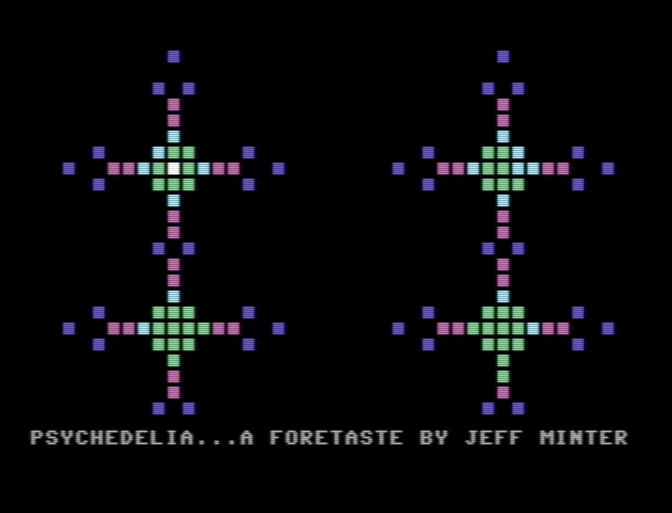
\includegraphics[height=5cm]{src/listing_commentary/four_pattern.png}
  \caption*{The display with \icode{currentSymmetrySettingForStep} set to \icode{\$02}}
\end{figure}


\clearpage
\begin{lstlisting}
presetColorValuesArray
;         0    6    2    4      5    3     7      1
  .BYTE BLACK,BLUE,RED,PURPLE,GREEN,CYAN,YELLOW,WHITE
;-------------------------------------------------------
; PaintPixel
;-------------------------------------------------------
PaintPixel   
        LDA pixelXPosition
        AND #$80 ; Detect if has moved off left of screen
        BNE ReturnEarly
        LDA pixelXPosition
        CMP #NUM_COLS
        BPL ReturnEarly
        LDA pixelYPosition
        AND #$80 ; Detect if has moved off top of screen.
        BNE ReturnEarly
        LDA pixelYPosition
        CMP #NUM_ROWS
        BPL ReturnEarly

        JSR LoadXAndYPosition
        LDA (currentLineForPixelInColorRamLoPtr),Y
        AND #COLOR_MAX

        LDX #$00
b408C   CMP presetColorValuesArray,X
        BEQ b4096
        INX 
        CPX #COLOR_MAX + 1
        BNE b408C

b4096   TXA 
        STA indexOfCurrentColor
        LDX currentValueInColorIndexArray
        INX 
        CPX indexOfCurrentColor
        BEQ ActuallyPaintPixel
        BPL ActuallyPaintPixel
        RTS 

ActuallyPaintPixel   
        LDX currentValueInColorIndexArray
        LDA presetColorValuesArray,X
        STA (currentLineForPixelInColorRamLoPtr),Y
        RTS 
\end{lstlisting}
\clearpage


\clearpage
\begin{lstlisting}
SetUpIntteruptHandlers   
        SEI 
        LDA #<MainInterruptHandler
        STA $0314    ;IRQ
        LDA #>MainInterruptHandler
        STA $0315    ;IRQ

        LDA #$0A
        STA cursorXPosition
        STA cursorYPosition

        LDA #$01
        STA $D015    ;Sprite display Enable
        STA $D027    ;Sprite 0 Color
        CLI 
        RTS 
\end{lstlisting}
\begin{lstlisting}
LoadXAndYPosition   
        LDX pixelYPosition
        LDA colorRAMLineTableLoPtrArray,X
        STA currentLineForPixelInColorRamLoPtr
        LDA colorRAMLineTableHiPtrArray,X
        STA currentLineForPixelInColorRamHiPtr
        LDY pixelXPosition
        RTS 
\end{lstlisting}
\begin{lstlisting}
LoadXAndYOfCursorPosition   
        LDX cursorYPosition
        LDA colorRAMLineTableLoPtrArray,X
        STA currentLineForCursorInColorRamLoPtr
        LDA colorRAMLineTableHiPtrArray,X
        STA currentLineForCursorInColorRamHiPtr
        LDY cursorXPosition
        RTS 
\end{lstlisting}
\begin{lstlisting}
PaintCursorAtCurrentPosition   
        JSR LoadXAndYOfCursorPosition
        LDA currentColorToPaint
        STA (currentLineForCursorInColorRamLoPtr),Y
        RTS 
\end{lstlisting}
\clearpage

Populate a table of hi/lo ptrs to the color RAM
of each line on the screen (e.g. \icode(\$D800), \icode(\$D828), \icode(\$D850) etc). Each entry represents a single
line 40 bytes long and there are twenty five lines.
The last line is reserved for configuration messages.




\clearpage
\begin{lstlisting}
MainInterruptHandler   
        DEC countStepsBeforeCheckingJoystickInput
        BEQ b4353
        JMP RETURN_FROM_INTERRUPT

b4353   LDA #$02
        STA countStepsBeforeCheckingJoystickInput
        LDA #$00
        STA currentColorToPaint

        JSR PaintCursorAtCurrentPosition
        LDA $DC00    ;CIA1: Data Port Register A
        AND #$03
        CMP #$03
        BEQ CheckIfCursorMovedLeftOrRight

        CMP #$02
        BEQ PlayerHasPressedDown

        ; Player has pressed up. Incremeent up two lines
        ; so that when we decrement down one, we're still
        ; one up!
        INC cursorYPosition
        INC cursorYPosition

PlayerHasPressedDown   
        DEC cursorYPosition
        LDA cursorYPosition
        CMP #$FF
        BNE CheckIfCursorAtBottom

        ; Cursor has reached the top of the screen, so loop
        ; around to bottom.
        LDA #$17
        STA cursorYPosition
        JMP CheckIfCursorMovedLeftOrRight

CheckIfCursorAtBottom   
        CMP #NUM_ROWS
        BNE CheckIfCursorMovedLeftOrRight
        ; Cursor has reached the bottom of the screen, so loop
        ; around to top
        LDA #$00
        STA cursorYPosition

\end{lstlisting}
\clearpage

Populate a table of hi/lo ptrs to the color RAM
of each line on the screen (e.g. \icode(\$D800), \icode(\$D828), \icode(\$D850) etc). Each entry represents a single
line 40 bytes long and there are twenty five lines.
The last line is reserved for configuration messages.



\clearpage
\begin{lstlisting}
CheckIfCursorMovedLeftOrRight   
        LDA $DC00    ;CIA1: Data Port Register A
        AND #$0C
        CMP #$0C
        BEQ CheckIfPlayerPressedFire

        CMP #$08
        BEQ CursorMovedLeft

        ; Player has pressed right.
        INC cursorXPosition
        INC cursorXPosition
CursorMovedLeft   
        DEC cursorXPosition
        LDA cursorXPosition
        CMP #$FF
        BNE CheckIfCursorAtExtremeRight

        LDA #$27
        STA cursorXPosition
        JMP CheckIfPlayerPressedFire

CheckIfCursorAtExtremeRight   
        CMP #NUM_COLS
        BNE CheckIfPlayerPressedFire
        LDA #$00
        STA cursorXPosition

CheckIfPlayerPressedFire   
        LDA $DC00    ;CIA1: Data Port Register A
        AND #$10
        BEQ PlayerHasntPressedFire

        LDA #$00
        STA stepsSincePressedFire
        JMP DrawCursorAndReturnFromInterrupt

\end{lstlisting}
\clearpage

Populate a table of hi/lo ptrs to the color RAM
of each line on the screen (e.g. \icode(\$D800), \icode(\$D828), \icode(\$D850) etc). Each entry represents a single
line 40 bytes long and there are twenty five lines.
The last line is reserved for configuration messages.


\clearpage
\begin{lstlisting}
PlayerHasntPressedFire   
        LDA stepsExceeded255
        BEQ b43D7
        LDA stepsSincePressedFire
        BNE DrawCursorAndReturnFromInterrupt

        INC stepsSincePressedFire
b43D7   INC indexIntoArrays
        LDA indexIntoArrays
        AND MAX_INDEX_VALUE
        STA indexIntoArrays

UpdateColorIndexArray  
        TAX 
        LDA currentColorIndexArray,X
        CMP #$FF
        BNE DrawCursorAndReturnFromInterrupt

        LDA cursorXPosition
        STA pixelXPositionArray,X
        LDA cursorYPosition
        STA pixelYPositionArray,X
        LDA #COLOR_MAX
        STA currentColorIndexArray,X

        LDA smoothingDelay
        STA initialFramesRemainingToNextPaintForStep,X
        STA framesRemainingToNextPaintForStep,X

DrawCursorAndReturnFromInterrupt   
        JSR LoadXAndYOfCursorPosition
        LDA (currentLineForCursorInColorRamLoPtr),Y
        AND #COLOR_MAX
        STA lastColorPainted
        LDA #WHITE
        STA currentColorToPaint
        JSR PaintCursorAtCurrentPosition
        JMP RETURN_FROM_INTERRUPT

\end{lstlisting}
\clearpage

Populate a table of hi/lo ptrs to the color RAM
of each line on the screen (e.g. \icode(\$D800), \icode(\$D828), \icode(\$D850) etc). Each entry represents a single
line 40 bytes long and there are twenty five lines.
The last line is reserved for configuration messages.

